\chapter{基于双通道注意力的极化SAR目标分类}
\section{引言}
极化SAR通过以不同的极化方式发射和接收电磁波信号,从而实现对地物目标探测,并提供丰富的后向散射信息。通过使用四种极化方式(HH、HV、VH、VV)进行探测,可以获得包含目标散射特性的散射矩阵。使用具有不同物理含义的散射基进行进一步解析,可以获取代表目标不同散射意义的目标分解特征。不同的极化特征从不同的角度描述地物目标的散射特性。挖掘极化SAR数据中的有效极化信息一直是遥感探测领域的难点与重点之一。通过采用适合于极化SAR数据特性的特征提取技术,可以使极化特征具有良好的类内相聚、类间远离的可分性,从而提升系统对目标特性的感知能力,成为极化SAR图像解译研究中的关键步骤之一。

根据文献\cite{刘高峰2014极化,1017062722.nh,1021744178.nh},没有一个单一特征能在所有分类中均取得完美的表现,每个方法提取的特征具有其长处以及特征见具有互补性。而目前在极化SAR目标分类研究中,主要存在以下问题:首先,现有的部分极化SAR分类方法直接采用相干矩阵作为输入,却忽略了目标分解特征的表示方式\citing{zhou2016polarimetric,liu2018polarimetric}提供的目标物理散射信息。其次,同一目标具有的多个极化特征也意味着存在较强的相关和冗余,且固定的极化特征表示方式无法应用在多元的目标分类场景中,导致目标分类性能受到限制\citing{ren2021mutual}。

针对上述问题,本章提出了一种基于双通道注意力的极化SAR目标分类方法。该方法以注意力机制为基础,通过利用极化散射特征与极化目标分解特征之间的差异性与互补性,构建了两种类型特征之间的融合表征关系,从而增强了极化信息的表征性能,并提高了分类任务的准确率。实验部分通过两组实测极化SAR数据验证本方法的有效性与优越性。

\section{注意力机制介绍}
\label{sec:sce3_1}
注意力机制是机器学习和深度学习中一种关键的技术,其主要目标是在处理信息是实现对输入数据的加权关注,以便网络模型能够更有效地捕捉与任务相关的信息。基于注意力机制的信息提取在自然语言处理、计算机视觉等领域获得了广泛的应用\citing{hu2018squeeze,vaswani2017attention}。注意力机制使用不同的权重来表示输入特征的不同的重要程度,根据关注的角度差异,可以分为通道注意力、空间注意力和混合注意力三种类型。
\subsection{通道注意力机制}
输入深度网络的特征一般使用多维数据表示,通道注意力专注于挖掘不同通道间的关键,通过自适应地调整通道之间的权重,使网络模型能够更加聚焦于对后续任务有益的特征通道,从而提升模型的性能和泛化能力。压缩和激励网络(Squeeze-and-Extraction Networks, SENet)\citing{hu2018squeeze}是最具代表性的通道注意力实现模型。图\ref{SENet}为SENet的组成结构图,该方法由压缩和激励两个阶段构成。在压缩阶段,通过全局池化操作对输入多维特征进行压缩,将每个通道的信息整合成单一的数值,用于全局感受野的建模。对于维数是$H\times W \times C$的输入特征,压缩操作将其压缩为$1 \times 1 \times C$维,具体如下式所示:
\begin{equation}
    z_c=\mathbf{F}_{sq}\left( \mathbf{u}_c \right) =\frac{1}{H\times W}\sum_{i=1}^H{\sum_{j=1}^W{u\left( i,j \right)}}
\end{equation}

在激励阶段,利用全连接层和激活函数,学习得到每个通道的权重。得到的权重向量用来对原始输入特征图中的每个通道进行加权,形成加权的特征图。具体如下式所示:
\begin{equation}
    \mathbf{s}=\mathbf{F}_{ex}\left( \mathbf{z},\mathbf{W} \right) =\sigma \left( g\left( \mathbf{z},\mathbf{W} \right) \right) =\sigma \left( \mathbf{W}_2\sigma *\left( \mathbf{W}_1\mathbf{z} \right) \right)
\end{equation}
其中,$\sigma$表示ReLu激活函数\citing{nair2010rectified},$W_1 \in \mathbb{R}^{\frac{C}{r}\times C}$且$W_2 \in \mathbb{R}^{C \times \frac{C}{r}}$。

模型最终通过权重向量$s$来对输入进行重标定得到:
\begin{equation}
    \widetilde{\mathbf{x}}_c=F_{scale}\left( \mathbf{u}_c,s_c \right) =s_c\mathbf{u}_c
\end{equation}
其中,$ \widetilde{\mathbf{X}}=\left[ \widetilde{\mathbf{x}_1},\widetilde{\mathbf{x}_2},\cdots ,\widetilde{\mathbf{x}_C} \right] $, $F_{scale}\left( \mathbf{u}_c,s_c \right)$ 表示 $s_c$与特征图$\mathbf{u}_c \in \mathbb{R}^{H\times W}$的通道级乘积。


\begin{figure}[h]
    \centering
    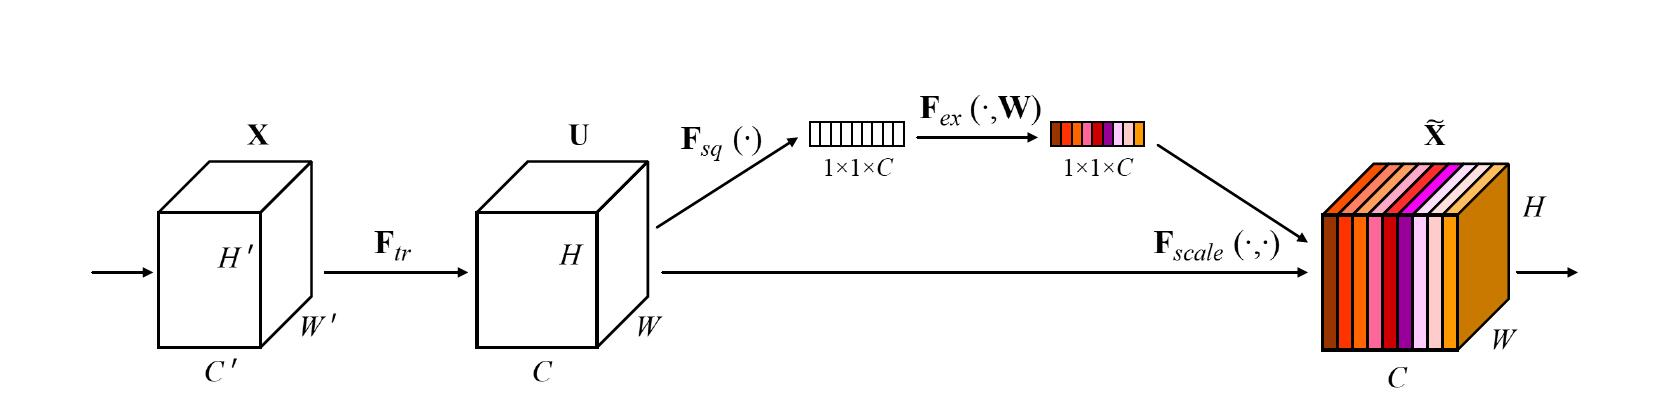
\includegraphics[width=14cm]{pic/chapter3/SENet.jpg}
    \caption{SENet 结构图\citing{hu2018squeeze}}
    \label{SENet}
\end{figure}

\subsection{空间注意力机制}
空间注意力机制是深度学习处理图像和空间数据中的注意力机制方法。其主要目的是通过对输入数据的不同空间位置引入不同的权重,赋予模型具备灵活关注对下游任务重要的区域的能力,提升模型对空间结构的感知能力。空间注意力模块(Spatial Attention Module, SAM)\citing{woo2018cbam}是一个经典的运用空间注意力机制的方法。如图\ref{SAM}所示,SAM的主要思想是首先利用最大池化层和平均池化层获得两个全局的特征图,然后通过拼接操作将两个特征图进行拼合,再利用一个$7\times 7$的卷积核将拼合的特征图转化成单通道的特征,最后使用sigmoid激活函数\citing{kyurkchiev2015sigmoid}得到空间注意力权值,并与原始输入进行相乘得到最终大小与输入相同的输出。空间注意力的计算公式如下式所示:
\begin{equation}
    \begin{aligned}
        \mathbf{M}_{\mathbf{s}}\left( \mathbf{F} \right) & =\sigma \left( f^{7\times 7}\left( \left[ AvgPool\left( \mathbf{F} \right) ;MaxPool\left( \mathbf{F} \right) \right] \right) \right)
        \\
                                                         & =\sigma \left( f^{7\times 7}\left( \mathbf{F}_{\mathbf{avg}}^{\mathbf{s}};\mathbf{F}_{\mathbf{max}}^{\mathbf{s}} \right) \right)
    \end{aligned}
\end{equation}

\begin{figure}[h]
    \centering
    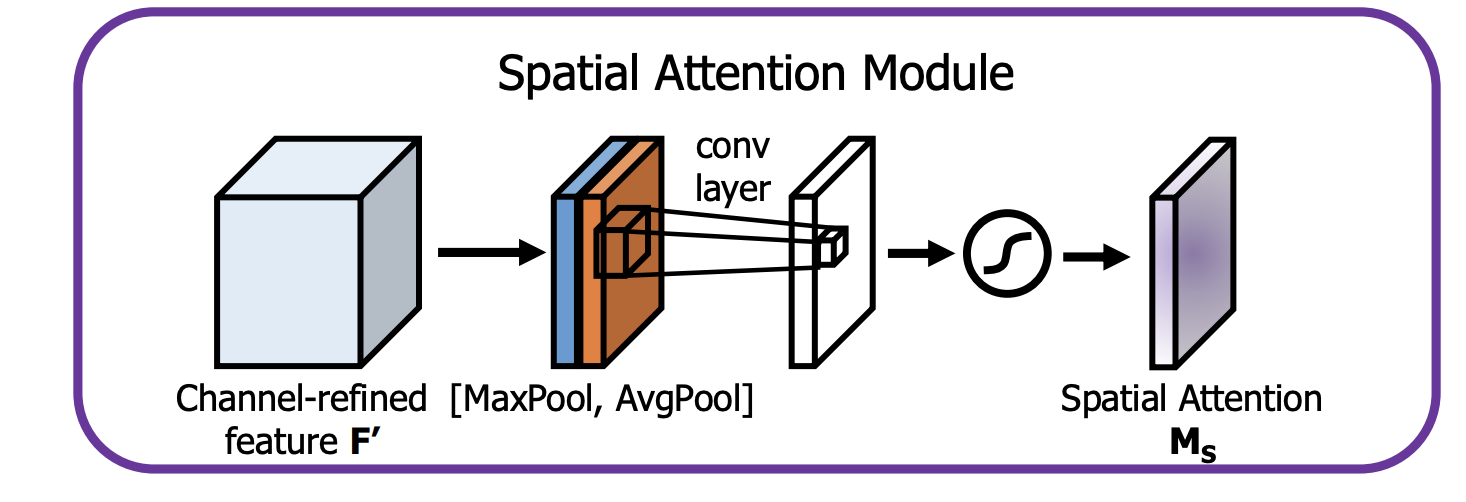
\includegraphics[width=12cm]{pic/chapter3/SAM.png}
    \caption{SAM 结构图\citing{woo2018cbam}}
    \label{SAM}
\end{figure}
\subsection{混合注意力机制}
混合注意力机制是综合多个注意力模块来处理数据的方法,通过对多个不同类型的注意力机制的融合,来增强深度网络模型对输入数据的建模能力,以更加灵活、全面地捕获输入数据的关键信息。卷积块注意力模块(Convolutional Block Attention Module, CBAM)\citing{woo2018cbam}是一个综合了通道和空间注意力机制的经典混合注意力方法。如图\ref{CBAM}所示,CBAM的主要网络架构有串联的通道注意力模块和空间注意力模块构成。通过依次使用通道和空间注意力模块,分别在通道和空间维度学习数据的关键信息,增强模型对输入数据的感知能力。其中,上一小节已经介绍了空间注意力模块的计算流程,而通道注意力机制的计算公式可以表示如下:
\begin{equation}
    \begin{aligned}
        \mathbf{M}_c\left( \mathbf{F} \right) & =\sigma \left( MLP\left( AvgPool\left( \mathbf{F} \right) \right) +MLP\left( MaxPool\left( \mathbf{F} \right) \right) \right)
        \\
                                              & =\sigma \left( \mathbf{W}_1\left( \mathbf{W}_0\left( \mathbf{F}_{avg}^{c} \right) \right) +\mathbf{W}_1\left( \mathbf{W}_0\left( \mathbf{F}_{max}^{c} \right) \right) \right)
    \end{aligned}
\end{equation}
其中,$\sigma$表示sigmoid函数,$W_0 \in \mathbb{R}^{C/r\times C}$、$W_1 \in \mathbb{R}^{C\times C/r}$均是多层感知机的权重参数。

因此,CBAM的计算流程可以表示为:
\begin{align}
    \mathbf{F}\prime=\mathbf{M}_{\mathbf{c}}\left( \mathbf{F} \right) \otimes \mathbf{F}
    \\
    \mathbf{F}''=\mathbf{M}_{\mathbf{S}}\left( \mathbf{F}\prime \right) \otimes \mathbf{F}\prime
\end{align}
其中,$\otimes$表示逐元素乘法。

\begin{figure}[h]
    \centering
    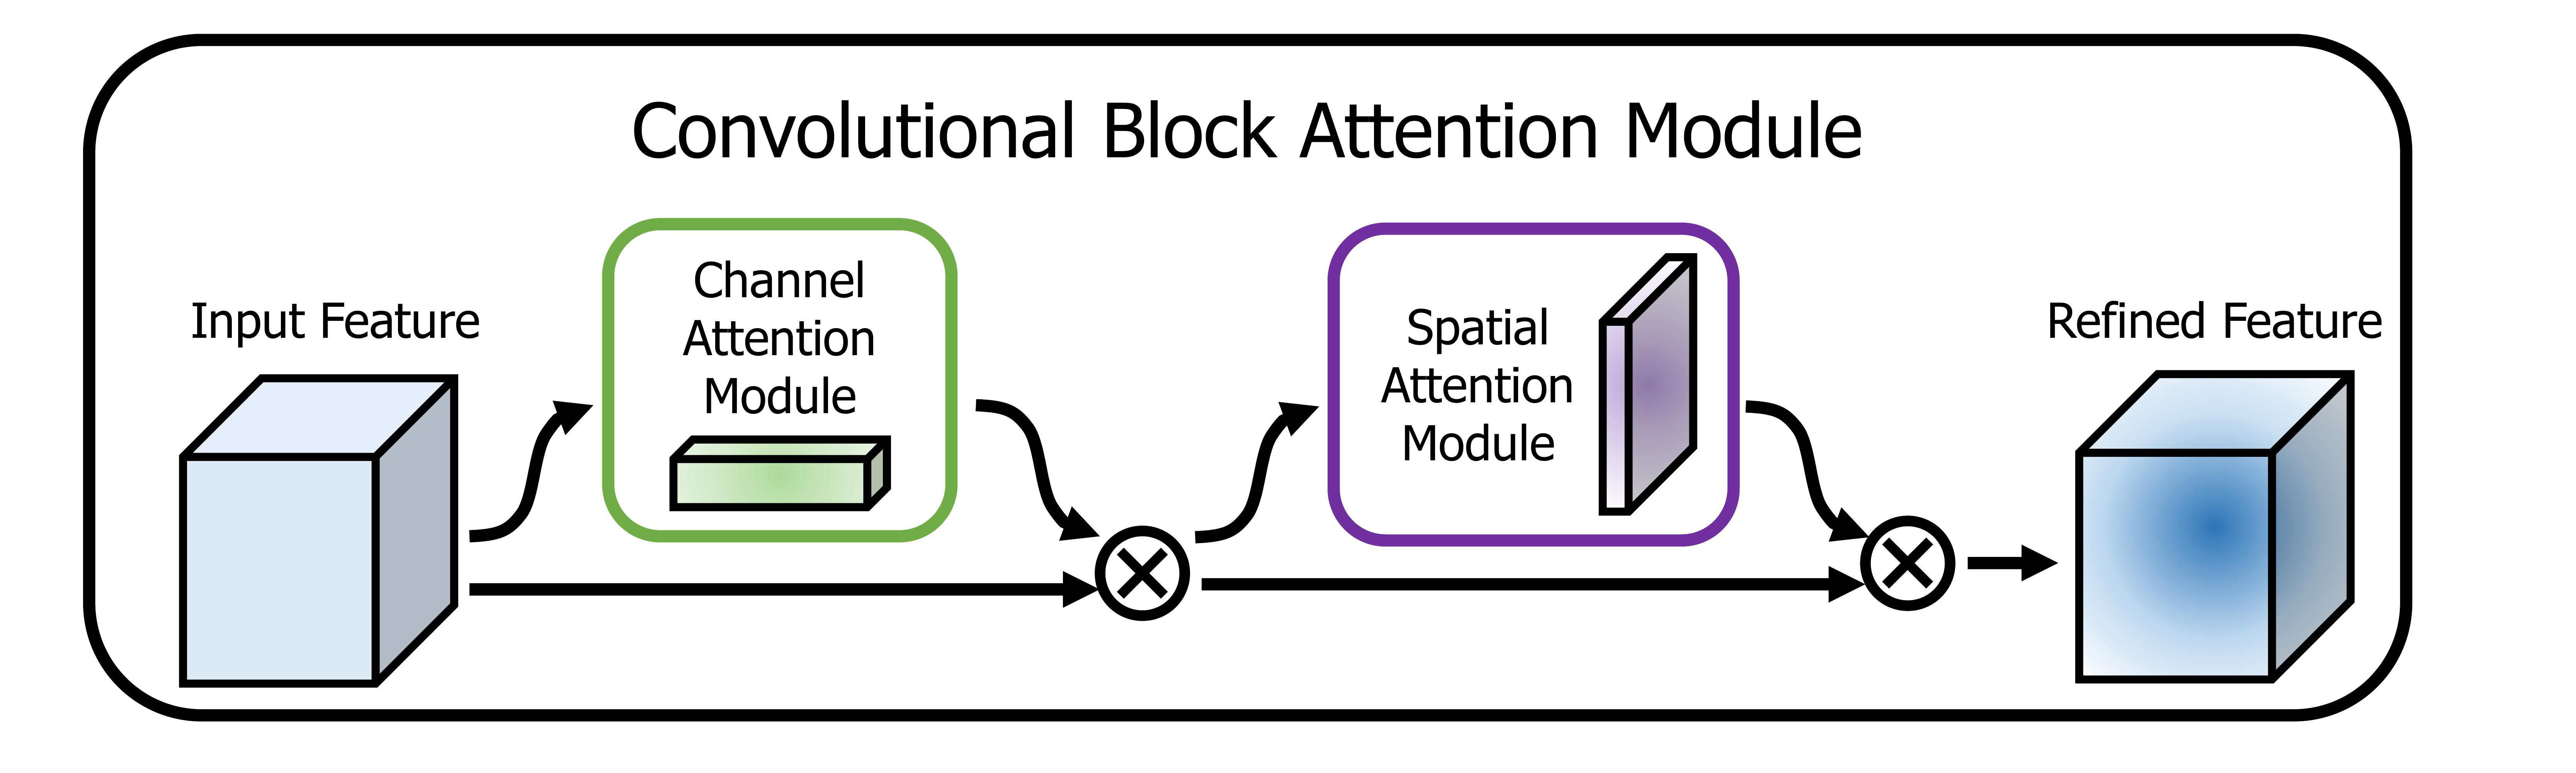
\includegraphics[width=12cm]{pic/chapter3/CBAM.jpg}
    \caption{CBAM 结构图\citing{woo2018cbam}}
    \label{CBAM}
\end{figure}

\section{双通道注意力的极化SAR目标分类}
注意力机制方法已广泛应用于图像处理领域,尤其在计算机视觉和深度学习任务中。这些方法通过在网络结构中引入注意力机制,对图像中特定区域进行加权关注,使模型能够更加关注关键的信息,从而提升分类性能。区别于光学图像,极化SAR图像具有独特的数据特征,包括复杂的多通道信息和多维度的散射机制,直接将通用的注意力机制方法应用于极化SAR图像处理任务中无法取得理想的效果。本章充分考虑了极化SAR图像数据特点,基于后向散射信息与目标分解信息的差异性与互补性,提出了专适用于极化SAR图像的目标分类方法,即基于双通道注意力的极化SAR目标分类方法。该方法充分挖掘两类极化特征的差异信息与互补信息,以提供更加全面、充分的极化信息表示方式,从而提升分类准确率。

\subsection{目标分类方法框架}
如图\ref{DPEN_framework}所示,展示了基于双通道注意力的极化SAR目标分类算法示意图。该方法构建了端到端的极化特征校准与分类网络结构,以挖掘多类型极化特征中的隐藏信息为目的,实现两类型极化特征的信息提取与有效融合,增强极化特征的可表征性能。

该方法主要分为极化特征校准模块与分类器模块,分别用于多类型极化特征细化以及目标分类任务。其主要思路是:首先,为了充分挖掘两类不同类型极化特征的有效信息,设计双通道网络结构,在两个独立的通道中依次利用注意力方法增强有效信息而抑制无关冗余信息。其次,利用极化注意力调整模块,基于两类型特征的互补特性,对空间和通道注意力图进行联合动态修正,充分挖掘两类极化特征之间的互补信息。之后, 考虑到极化SAR图像具有较大的空间尺寸,设计多尺度学习方法,旨在聚合不同尺寸的极化特征。最后,将重新调整的极化特征进行拼接,形成注意力增强的极化特征输入到分类器网络,得到目标分类结果。值得注意的是,该方法中的极化特征校准模块可以作为一个即插即用的插件式模块,应用到其他下游的目标检测、分类识别任务中。

\begin{figure}[ht!]
    \centering
    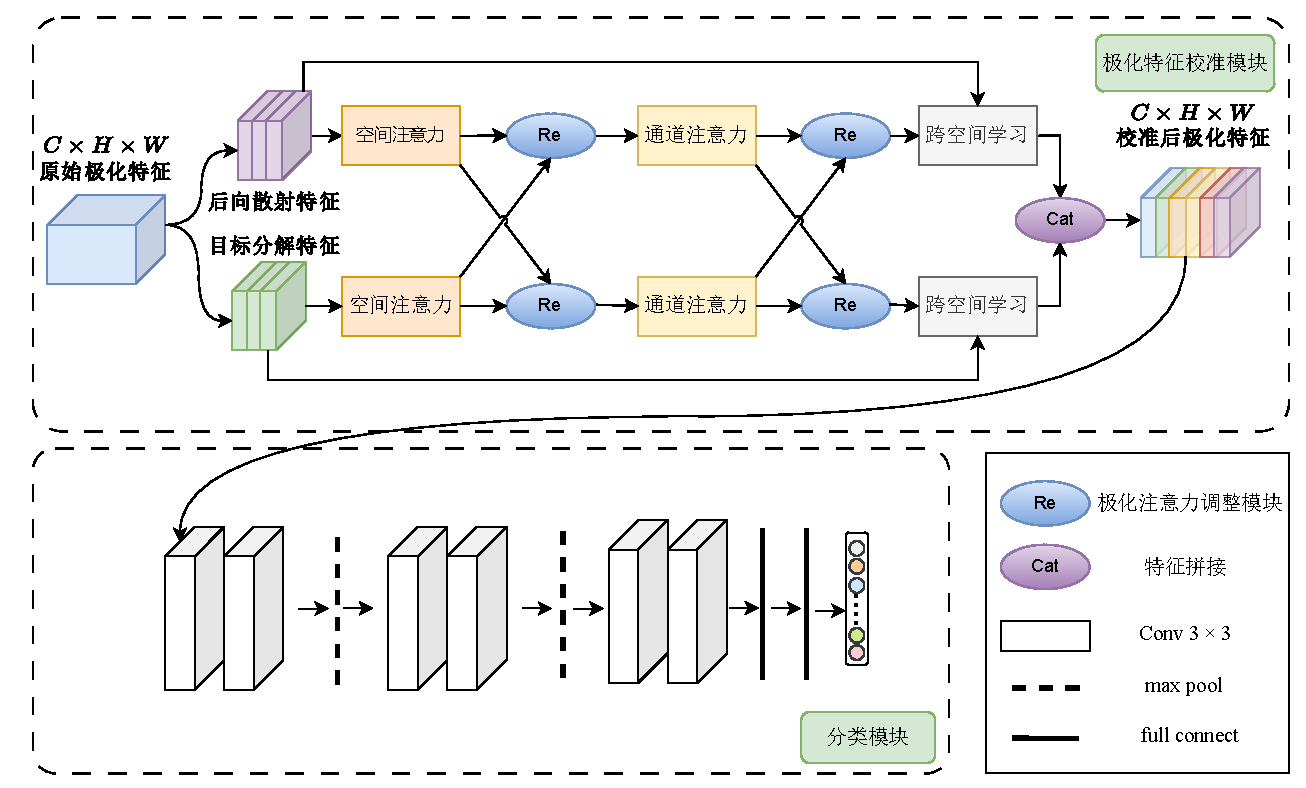
\includegraphics[width=14cm]{pic/chapter3/基于双通道注意力的极化SAR分类方法.pdf}
    \caption{基于双通道注意力的极化SAR分类方法示意图}
    \label{DPEN_framework}
\end{figure}

极化特征校准模块输入结构呈现两个独立通道形式,分别输入具有目标完备后向散射信息的极化相干矩阵和具有不同物理散射特性的极化目标分解特征。两路分支输入特征如下所示:

(1)通道1:后向散射特征

根据公式\eqref{eq:T},极化相干矩阵$T$非主对角线元素均是复数,而主对角线元素均是实数,并且关于主对角线共轭对称。因此,可以使用矩阵的上三角6个元素代表极化相干矩阵,考虑到复数性质,使用一个包含9个元素的一维数组表示极化相干矩阵,具体如下式所示:
\begin{equation}
    \mathbf{V}=[T_{11}, T_{22}, T_{33}, \text{Re}(T_{12}), \text{Re}(T_{13}), \text{Re}(T_{23}), \text{Im}(T_{12}), \text{Im}(T_{13}), \text{Im}(T_{23})]
\end{equation}
其中,$\text{Re}$与$\text{Im}$分别表示取实部与取虚部运算。$\mathbf{V}$包含了地物目标完备的后向散射信息,将$\mathbf{V}$作为通道1的输入。

(2)通道2:目标分解特征

不同的极化目标分解特征从不同的物理层面反映了目标的散射特性,通道2选择多种经典的极化目标分解特征作为输入,分别为Pauli分解、Cloude分解、Freeman分解、Krogager分解、Huynen分解共计32维目标分解参数。具体特征参数如表\ref{tab:decomposition_features}所示。

% Please add the following required packages to your document preamble:
% \usepackage{multirow}
\begin{table}[ht!]
    \caption{通道2使用的极化目标分解特征参数表}
    \label{tab:decomposition_features}
    \centering
    \begin{tabular}{|c|c|c|c|}
        \hline
        分解方法                     & 特征参数                                                             & 物理意义               & 特征维数 \\ \hline
        Pauli                    & $\left| a \right|^2,\left| b \right|^2,\left| c \right|^2$       & 奇次、偶次、二面角散射        & 3    \\ \hline
        \multirow{2}{*}{Cloude}  & $H,\alpha,A$                                                     & 散射熵、平均散射角、反熵       & 3    \\ \cline{2-4}
                                 & $\lambda_1,\lambda_2,\lambda_3$                                  & 极化相干矩阵特征值          & 3    \\ \hline
        \multirow{2}{*}{Freeman} & $P_s,P_d,P_v,P_r$                                                & 表面散射、体散射、二次散射、同极化比 & 4    \\ \cline{2-4}
                                 & $f_s,f_d,f_v$                                                    & Freeman系数          & 3    \\ \hline
        Krogager                 & $\left| k_s \right|^2,\left| k_d \right|^2,\left| k_h \right|^2$ & 球、双平面、螺旋散射能量       & 4    \\ \hline
        \multirow{3}{*}{Huynen}  & $A_0,B_0+B,B_0-B$                                                & 对称、非对称、不规则性信息      & 3    \\ \cline{2-4}
                                 & $C,D,E$                                                          & 线性、弯曲、扭转性信息        & 3    \\ \cline{2-4}
                                 & $F,G,H$                                                          & 螺旋、沾合、方向信息         & 3    \\ \hline
        Van Zyl                  & $f_v,f_d,f_s$                                                    & 体散射、二次散射、表面散射系数    & 3    \\ \hline
    \end{tabular}
\end{table}

为了高效的提取单独通道内的有效极化信息,使用空间和通道注意力方法对输入的极化特征进行细化,以激发有效的重要信息而抑制无关的冗余信息,以加权的方式对输入极化特征进行校准。空间与通道注意力模块的具体网络结构及计算流程将在\ref{sec:空间和通道注意力模块}小节中介绍。

为了有效融合两类极化特征,挖掘双通道内不同特征的互补信息,设计了极化注意力修正模块,以极化信息一致性为引导,通过残差连接的形式,实现由一类极化信息到另一类极化信息的融合修正。极化注意力修正模块的具体网络结构及计算流程在\ref{sec:极化注意力修正模块}小节中介绍。

鉴于极化SAR目标具有空间尺寸差异大的特点,为了聚合不同尺寸的极化特征,设计了多尺度学习模块,以不同卷积核大小分的卷积层提取不同尺寸的空间信息,结合全局平均池化以及非线性函数映射操作,实现多尺度的极化特征学习。多尺度学习模块的具体网络结构及计算流程在\ref{sec:多尺度学习模块}小节中介绍。

最后,通过特征拼接,将校准后的两类型极化特征进行聚合后作为分类器模块输入,完成目标分类。

综合以上算法描述,图\ref{流程图}对本章算法结合分类器进行目标分类的整体流程进行总结。
\begin{figure}[ht!]
    \centering
    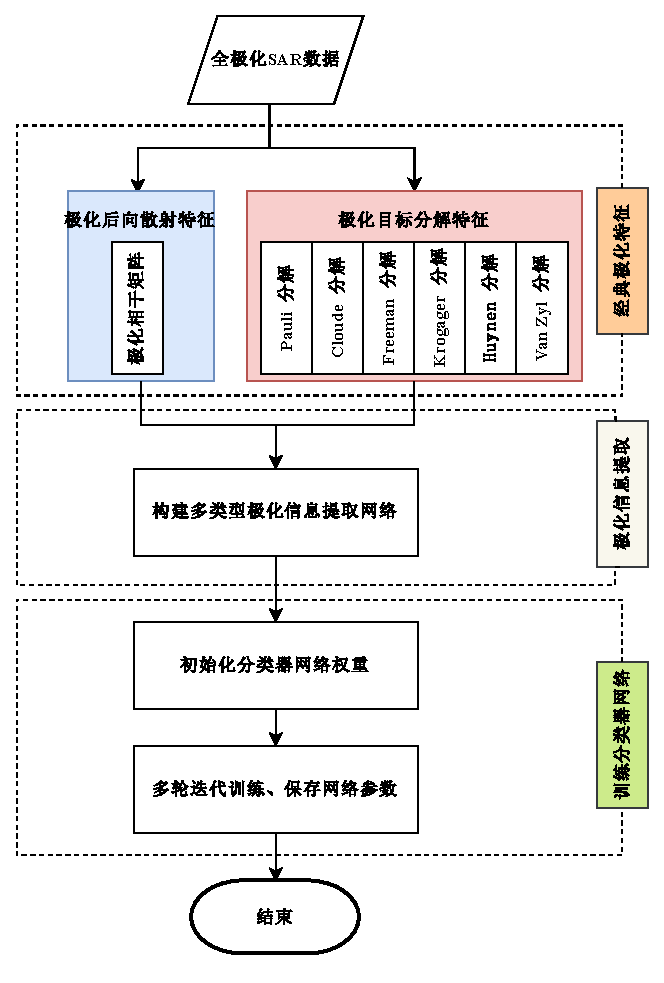
\includegraphics[width=10cm]{pic/chapter3/DP流程图.pdf}
    \caption{双通道注意力极化SAR目标分类算法流程图}
    \label{流程图}
\end{figure}

\subsection{空间和通道注意力模块}
注意力方法通过强调或抑制输入特征中的不同部分,在深度学习领域,被广泛应用到各种任务中。本文通过引入空间和通道注意力方法,旨在对输入的极化信息动态调整关注度,提升模型对关键信息的感知能力。图\ref{fig:spatial}为本方法中的空间注意力模块网络结构。空间注意力方法采用卷积操作来获取全局信息,从而赋予其更多的非线性捕捉能力,更好的拟合不同空间位置之间的复杂相关性,显著减少参数量和计算量。计算公式如下所示:
\begin{equation}
    A_s=\sigma(f^{7\times 7}(AvgPool(S);\Gamma(MaxPool(S))))
\end{equation}
其中,$f^{7\times 7}$表示卷积核大小为$7\times 7$的卷积操作;$\sigma$表示Sigmoid激活函数。空间注意力通过最大池化和平均池化两个池化操作得到大小为$2\times H \times W$的特征图,最大池化从图像中提取强的局部信息,平均池化提取全局平均统计特征。对特征图采用卷积运算,转换为$1\times H\times W$的单一通道特征,再利用Sigmoid激活函数将通道特征图转为对应的空间注意力图$A_s$,最后计算注意力图$A_s$与原始输入特征的乘积得到空间注意力信息。计算公式如下:
\begin{equation}
    S_S=A_S \otimes S
\end{equation}
其中,$\otimes$ 表示逐元素乘积。通过空间注意力方法,在空间维度进行有效信息激发而抑制无效信息,得到空间注意力图校准的极化特征$S_S$。

\label{sec:空间和通道注意力模块}
\begin{figure}[ht!]
    \centering
    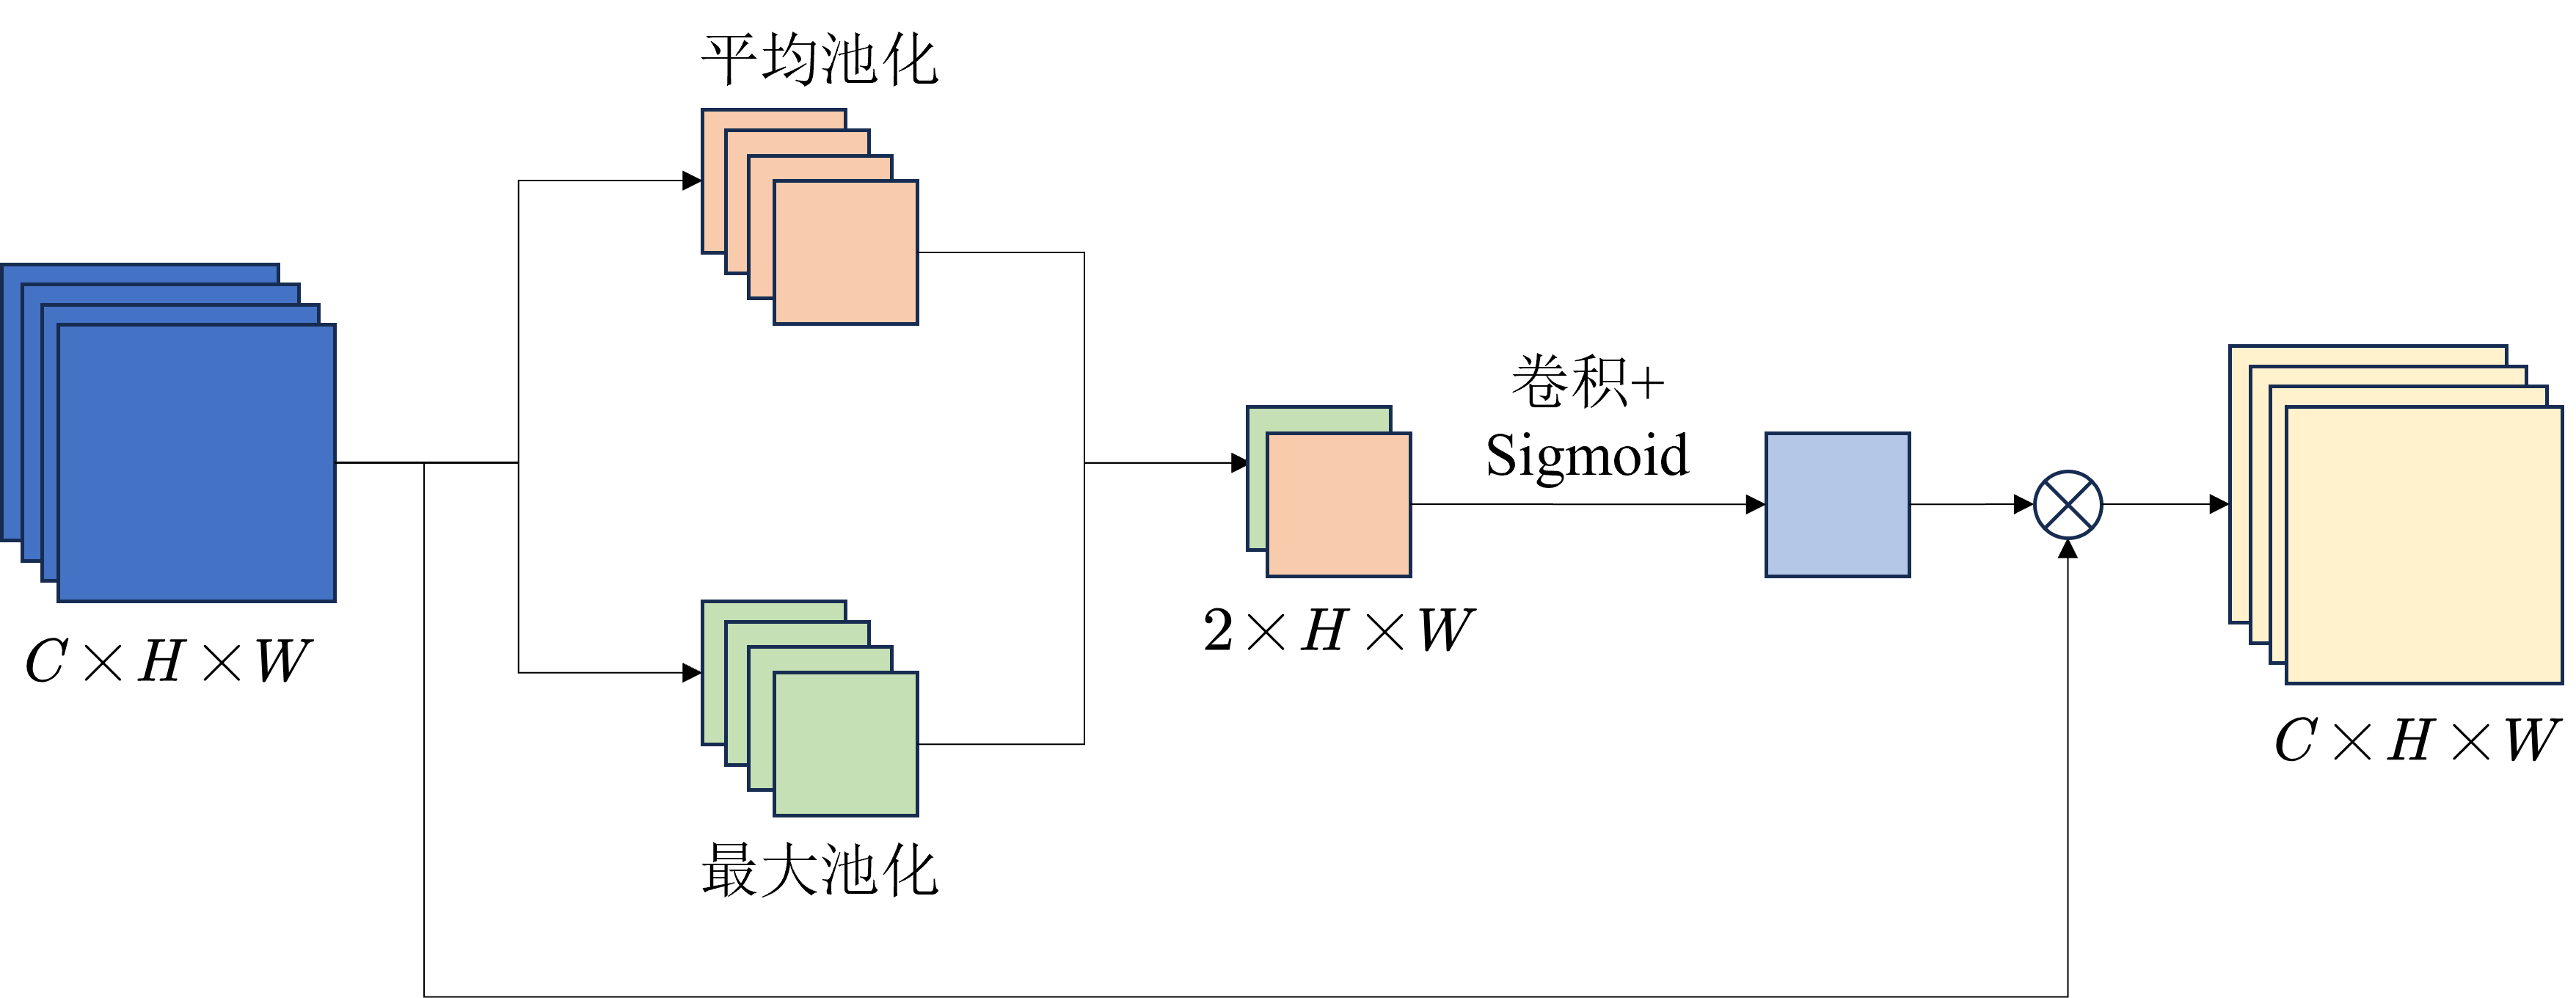
\includegraphics[width=14cm]{pic/chapter3/Spatial.png}
    \caption{空间注意力模块结构}
    \label{fig:spatial}
\end{figure}

相比于空间注意力方法使用卷积层层与激活函数的注意力提取方法,通道注意力方法通过全连接和加和操作,完成对通道维度信息的提取。全局最大池化与平均池化操作对输入特征图的空间依赖性进行拆解,并通过逐个学习每个通道生成反映各个通道重要性的特征图。随后,将得到的两个$C\times 1 \times 1$的特征图进行拼接后使用全连接和加和运算后,再使用Sigmoid激活函数,形成成一维的通道注意力图,用于表示不同通道特征图的重要性。计算如下式所示:
\begin{equation}
    A_C=\sigma(\Gamma(AvgPool(S))+\Gamma(MaxPool(S)))
\end{equation}
其中,$\sigma$表示Sigmoid激活函数;$\Gamma$表示两层神经网络。将通道注意力图与输入极化特征相乘,得到通道注意力图校准的极化特征。计算公式如下:
\begin{equation}
    S_C=A_C \otimes S
\end{equation}
其中,$\otimes$表示逐元素乘法。

\begin{figure}[ht!]
    \centering
    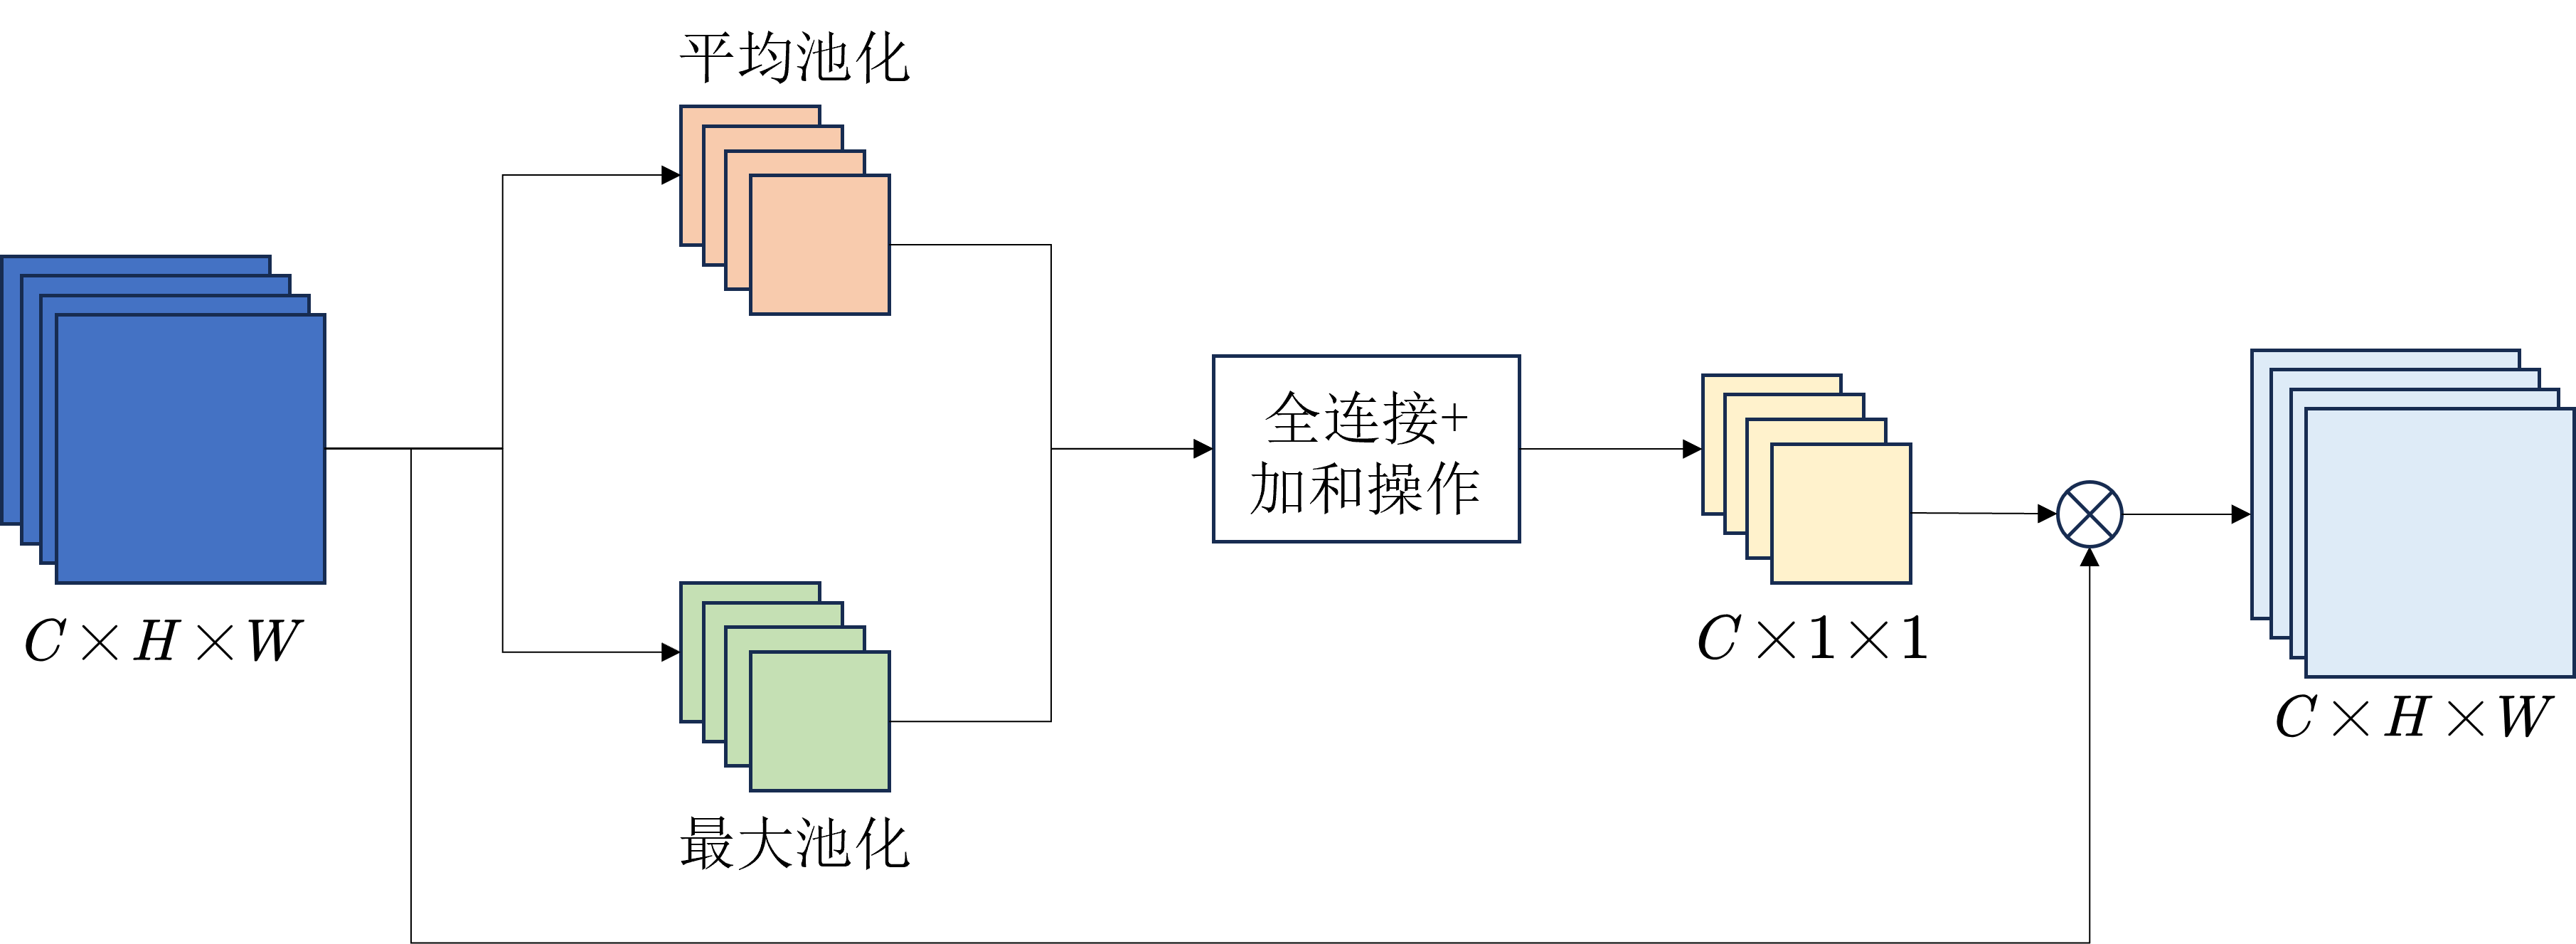
\includegraphics[width=14cm]{pic/chapter3/Channel.png}
    \caption{通道注意力模块结构}
    \label{fig:channel}
\end{figure}

\subsection{极化注意力修正模块}
\label{sec:极化注意力修正模块}

基于双通道注意力架构对极化SAR输入特征提取空间、通道注意力特征图,对于同一类型目标,校准后的两种类型极化信息存在一致性与互补性。为了保持特征一致性和挖掘极化互补信息,图\ref{DPEN_WFM}展示的极化注意力修正模块,以极化信息一致性为引导,对输入的极化特征进行动态调整,增强特征一致性。极化注意力修正模块利用极化特征估计特征映射的位置相关关系,自适应地控制两类注意力图的空间位置信息。以双通道的注意力图$S_1\in R^{H \times W}$与$S_2\in R^{H \times W}$为输入,该模块的计算流程可以表示为:
\begin{gather}
    S_{2}^{\prime}=f^{1\times 1}\left( S_2 \right)
    \\
    S_{1}^{\prime}=\mathrm{Ref}\left( S_{2}^{\prime},\varphi \left( S_1 \right) \right)
    \\
    S_{out}=S_{1}^{\prime}+S_1
\end{gather}
其中,$S_{out}$表示模块最终输出,运算$\varphi(\cdot)$表示在特征$S_1$引导下估计$S_2$的位置相关矩阵,描述了两路特征的空间对应关系,$\mathrm{Ref}(\cdot)$表示根据位置相关矩阵调整$S_{2}$,运算$\varphi(\cdot)$采用类似softmax运算操作计算归一化相关矩阵值,具体可以表示为:
\begin{equation}
    \Phi _i\left( j \right) =\frac{\exp \left( \theta \left( S_i \right) ^T\cdot \phi \left( S_j \right) \right)}{\sum_j{\exp \left( \theta \left( S_i \right) ^T\cdot \phi \left( S_j \right) \right)}}
\end{equation}
其中,$i$是指相关矩阵中某个位置的索引,$j$是枚举所有位置的索引。$\Phi_i(j)$描述了空间位置$i$与位置$j$之间的对应关系。$\theta(\cdot)$与$\phi(\cdot)$均使用卷积核大小为$1\times 1$的卷积层实现。

对于输入注意力特征图位置索引$i$处的特征单元,以对应位置的相关元素$\Phi_i$为引导,修正过程可以表示为:
\begin{equation}
    S_{1i}^{\prime}=\sum_j{\Phi _i\left( j \right) \cdot S_{2}^{\prime}\left( j \right)}
\end{equation}

\begin{figure}[h]
    \centering
    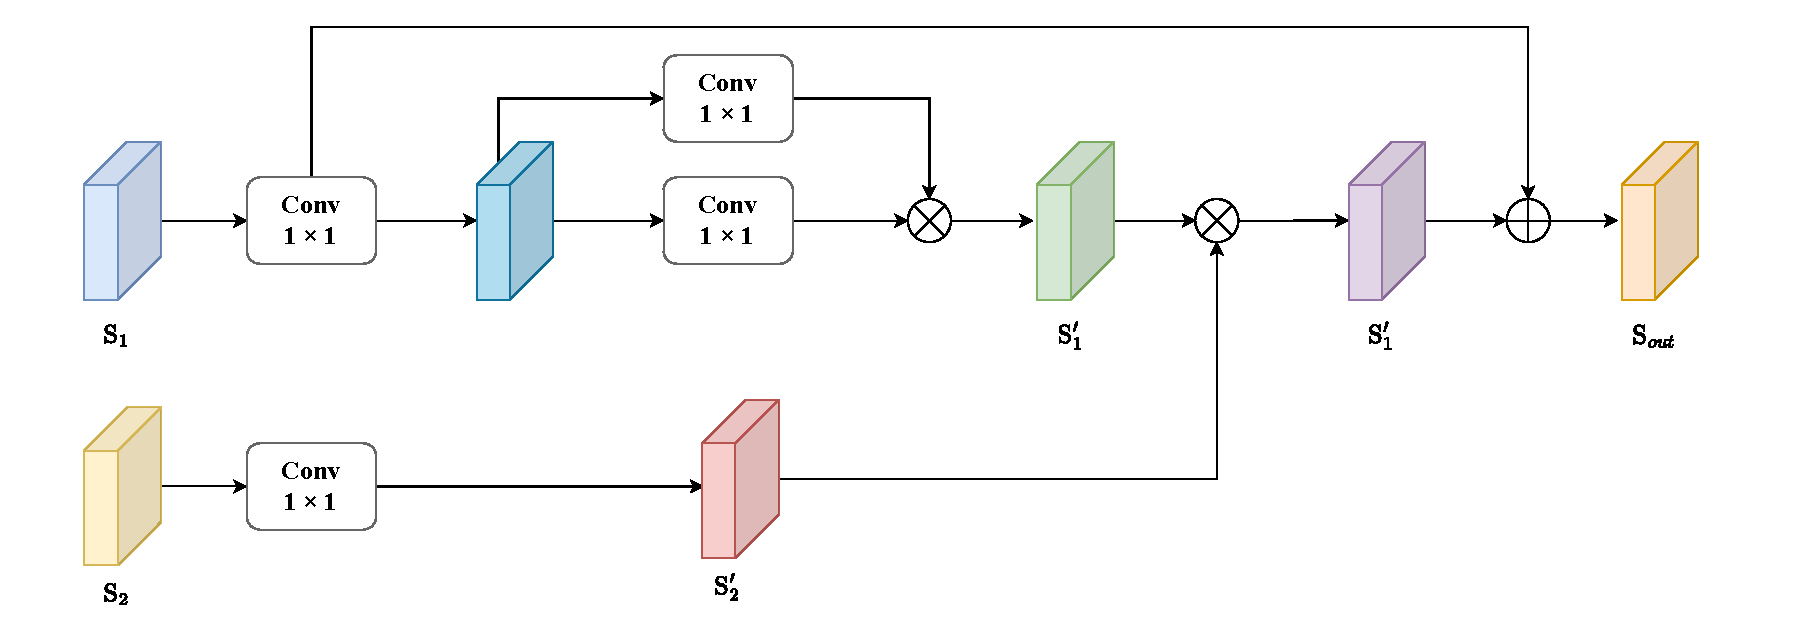
\includegraphics[width=14cm]{pic/chapter3/极化注意力修正.pdf}
    \caption{极化注意力修正模块网络结构示意图}
    \label{DPEN_WFM}
\end{figure}

% 极化注意力修正模块利用输入的一路极化特征作为主要引导,对另外一路特征进行修正。其中主要包含卷积与残差运算,计算公式如下所示:
% \begin{gather}
%     S_{1}^{\prime}=f^{1\times 1}\left( f^{1\times 1}\left( S_1 \right) \right) \times f^{1\times 1}\left( f^{1\times 1}\left( S_1 \right) \right)
%     \\
%     S_{2}^{\prime}=f^{1\times 1}\left( S_2 \right)
%     \\
%     S_{out}=S_1+\left( S_{1}^{\prime}\times S_{2}^{\prime} \right)
% \end{gather}



\subsection{多尺度学习模块}
\label{sec:多尺度学习模块}
\begin{figure}[ht!]
    \centering
    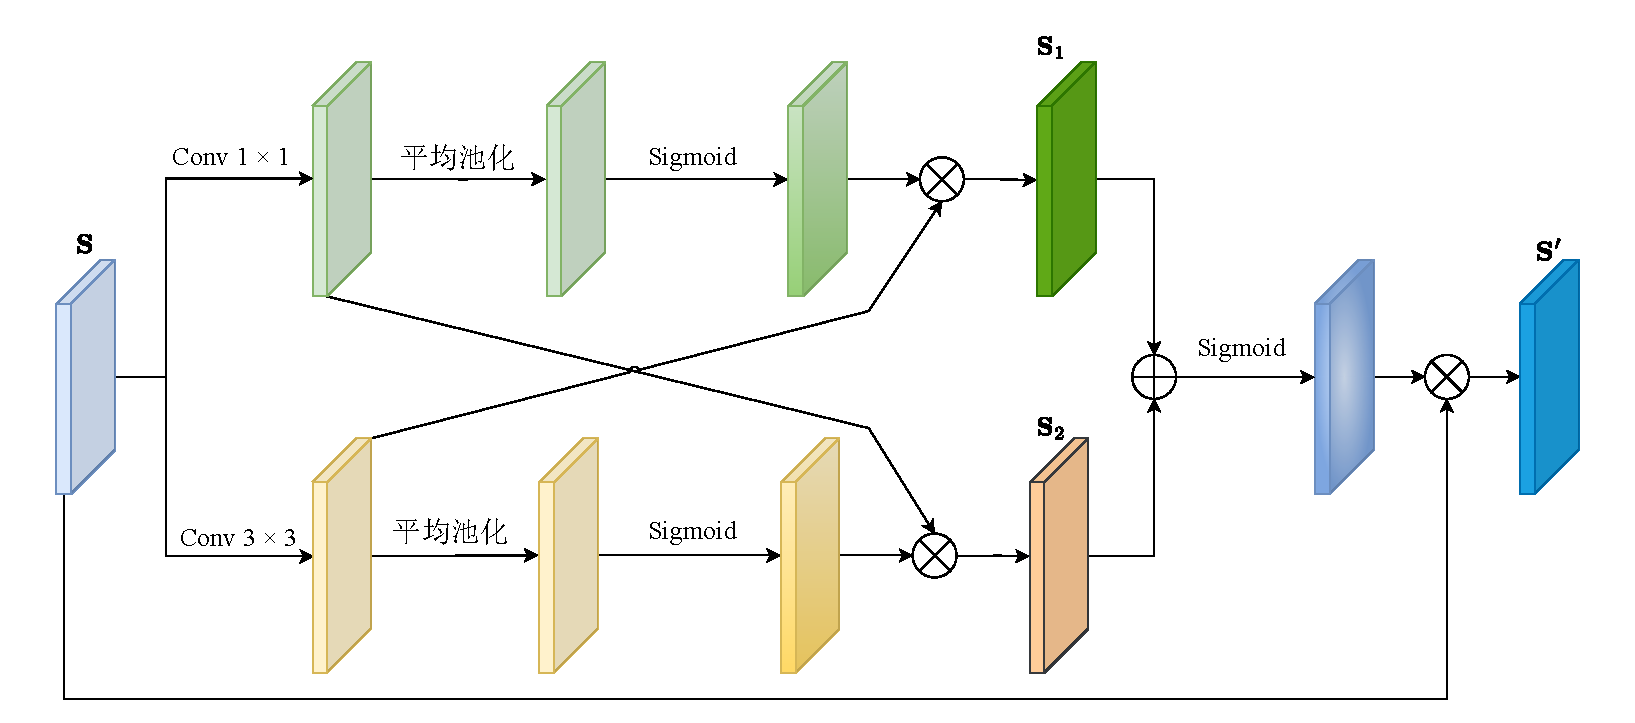
\includegraphics[width=14cm]{pic/chapter3/跨空间学习.pdf}
    \caption{多尺度学习模块网络结构示意图}
    \label{DPEN_CSL}
\end{figure}

多尺度学习模块的网络结构如图\ref{DPEN_CSL}所示,提供了一种不同空间维度方向的极化信息聚合方法,以实现多尺度下的极化特征聚合。引入两个分支的张量,分别代表了$1\times 1$分支的输出和$3 \times 3$分支的输出。通过二维全局平均池化对$1\times 1$分支的输出进行操作,以编码其中的全局极化空间信息,用于对全局信息进行编码和建模远程依赖关系。二维全局池化操作可以表达为:
\begin{equation}
    z_c=\frac{1}{H\times W}\sum_{j}^{H}\sum_{i}^{W}x_c(i,j)
\end{equation}

$1\times 1$分支特征图在进行二维全局平均池化后,采用自然非线性函数Softmax进行二维高斯映射,以拟合线性变换并提升计算效率。通过将上述并行处理的输出进行矩阵点积运算,并与结果相乘,得到了第一个空间注意力图。类似地,利用二维全局平均池化对$3\times 3$分支进行全局空间信息的编码。这会生成每组内输出特征的两个空间权重值的集合,随后使用Sigmoid函数将其映射为相应空间位置的权重关系,突出显示所有像素的全局上下文信息。计算公式如下:

在以上二维全局平均池化的输出处采用二维高斯映射的自然非线性函数Softmax来拟合线性变换,进而提升计算效率。通过将上述并行处理的输出与矩阵点积运算相乘,得出了第一个空间注意力图。同样利用二维全局平均池化在$3\times 3$分支编码全局空间信息,将每组内的输出特征映射计算为生成的两个空间权重值的集合,然后使用Sigmoid函数映射成空间位置对应的权重关系。通过捕获像素级的成对关系,突出显示所有像素的全局上下文信息。计算公式如下:
\begin{gather}
    S_1=f^{1\times 1}\left( S \right) \times \mathrm{AvgPool}\left( f^{3\times 3}\left( S \right) \right)
    \\
    S_2=f^{3\times 3}\left( S \right) \times \mathrm{AvgPool}\left( f^{1\times 1}\left( S \right) \right)
    \\
    S^{\prime}=\sigma \left( S_1+S_2 \right)
\end{gather}
其中,$\sigma$表示sigmoid函数。

\subsection{目标分类模块}
\label{sec:目标分类模块}
在双通道注意力极化信息提取器(Dual Attention Polarization Information Extractor, DP)的基础上,构建端到端的极化SAR信息提取与目标分类网络(DP Convolutional Neural Network, DP-CNN)。从输入的高维原始极化特征出发,利用DP模块可以获得全局信息并且嵌入到分类器中。原始极化特征中有价值的信息被激发,而没有价值的信息被抑制。当具备了重新校正的极化特征之后,输入到目标分类器模块,通过卷积网络结构,实现对输入特征的分类。校准后的极化特征输入到图\ref{DPEN_framework}展示的分类模块中。分类器采用类似VGG结构的卷积神经网络架构,其中包含三个带有ReLU激活函数的$3\times 3$卷积层、两层最大池化函数、两层全连接网络以及一层SoftMax激活层。

以交叉熵损失函数\citing{mao2023cross}为目标,通过反向传播算法训练模型参数。DP-CNN方法将输入的原始极化特征$x$映射为预测概率$p\in \mathbb{R}^{C}$,其中,$C$表示类别的个数。$x$对应的中心像素预测标签可以通过选择概率最高的类别,即向量$p$的最大值索引来预测。其计算公式如下:
\begin{equation}
    L=\sum_{i=1}^{n}p(x_i)\text{log}(q(x_i))
\end{equation}
其中,$p(x)$表示真实值分布概率,$q(x)$表示模型预测分布概率。交叉熵值的变化与模型的训练效果密切相关,优越的训练效果会让预测概率分布逐渐趋近于真实值概率分布,相应的交叉熵值会逐渐减少。

整个模型的损失计算流程可以表示为:

(1)神经网络分类器最后一层输出每个样本类别的属性值向量;

(2)利用Softmax函数将属性值向量映射为样本属于每一类的预测概率向量;

(3)地面真值标签的one hot编码与样本预测概率向量进行交叉熵损失函数运算,并依据损失值进行反向传播优化。


\section{实验结果与分析}
本节将详细阐述验证实验所依托的软件件设施配置以及关键的超参数设置。在此基础上,对验证实验所使用的极化SAR数据集进行简要介绍,并对本章所提出的双通道注意力目标分类方法进行性能评估。

\subsection{实验参数设置}
本章实验所使用的计算环境为一台CPU为Intel Core i7-8700K和配备了NVIDIA GPU(GeForce RTX 3090, 24G)的计算机设备。操作系统采用Ubuntu 20.04 LTS。深度学习框架选择PyTorch,版本为1.9.0,同时依赖CUDA深度神经网络库(cuDNN)版本8.0.5。在科学计算方面,实验使用NumPy库,版本为1.19.5。

学习率作为深度学习模型训练的关键参数之一,其值的选择对于模型的收敛速度至关重要。在训练过程中,如果学习率设置的过大或者过小,均会可能给模型的分类准确度产生负面影响。通常情况下,在模型的训练初始阶段,采用较大的学习率能够使模型快速收敛到最优点附近。随着训练的执行,逐渐减小学习率,以更加精确地接近最优点。在本章所采用的模型中,初始学习率为$3\times 10^{-4}$,在训练至第30至60个epoch期间,学习率经过衰减变为原值的0.1倍。这里的epoch表示训练集中素有样本完成一次正向传递和反向传播的过程,本章中模型训练的epoch设置为100。Batch size表示每次训练中选择的样本数量,其值的大小会影响网络的优化速度和执行效率。在本章模型中,batch size被设置为64。实验中,使用大小为$15 \times 15$,步长为1的滑动窗口对输入图像进行随机截取,选取出1\%的中心带标签样本作为训练集,而其余的样本作为测试集。

为了对本章提出的极化信息提取方法进行全面地评估和对比,从两个对比维度选择了多种替代方案进行比较:一是对特征输入的改变,二是对极化特征校准模块的替换。首先,验证了不同极化特征表示对目标分类任务的影响。对比方法包括仅使用极化相干矩阵中的元素结合CNN分类方法(记为CNN-T)、仅使用极化目标分解特征结合CNN分类方法(记为CNN-P)、以及基于散射特征和分解特征简单叠加结合CNN的分类方法(记为CNN-F)。这旨在验证本章方法在极化特征表示方面的有效性。其次,对极化特征校准模块进行替换。利用基于压缩和激励网络结合CNN分类方法(记为CNN-SE)和基于空间通道注意力结合CNN分类方法(记为CNN-CBAM)作为不同的对比方法。这旨在验证本章方法在极化特征表示方面的优越性。

\subsection{精度评价方法}
精度评价是对实际数据和模型分类结果进行比较的重要步骤,旨在确定分类模型的准确性,是衡量分类结果可靠性的关键指标。混淆矩阵(Confusion Matrix)通常作为遥感图像分类准确性能的评判指标,并且可以通过混淆矩阵计算得到多种常用的评价参数指标,包括
生产者精度(Producer Accuracy, PA)、使用者精度(User Accuracy, UA)、总体分类准确率(Overall Accuracy, OA)、平均分类准确率(Average Accuracy, AA)、Kappa系数等。

如表\ref{tab:conf_示意表}所示,c类样本混淆矩阵是一个$c \times c$的矩阵,其中$c$表示数据集的类别数量。混淆矩阵的行表示实际类别,列表示预测类别。其中,每个元素$(i, j)$表示实际属于类别$i$的样本被预测为类别$j$的数量。混淆矩阵主对角线元素表示被正确分类的样本,非主对角线表示分类错误的样本。

\begin{table}[ht!]
    \caption{c类样本混淆矩阵示意}
    \label{tab:conf_示意表}
    \centering
    \begin{tabular}{ccccccc}
        \hline
                                    &          & \multicolumn{4}{c}{地面真实类别} &                                           \\
        \cline{3-6}
                                    &          & 第 1 类                      & 第 2 类    & $\ldots$ & 第 $c$ 类  & 预测样本数    \\
        \multirow{4}{*}{预测类别}       & 第 1 类    & $n_{11}$                   & $n_{12}$ & $\ldots$ & $n_{1c}$ & $n_{1+}$ \\
                                    & 第 2 类    & $n_{21}$                   & $n_{22}$ & $\ldots$ & $n_{2c}$ & $n_{2+}$ \\
                                    & $\vdots$ & $\vdots$                   & $\vdots$ & $\ddots$ & $\vdots$ & $\vdots$ \\
                                    & 第 $c$ 类  & $n_{c1}$                   & $n_{c2}$ & $\ldots$ & $n_{cc}$ & $n_{c+}$ \\
        \multicolumn{2}{c}{地面真值样本数} & $n_{+1}$ & $n_{+2}$                   & $\ldots$ & $n_{+c}$ & $N$                 \\
        \hline
    \end{tabular}
\end{table}

在极化SAR图像分类结果精度评价中,可以基于混淆矩阵定义以下指标:

1.总体分类准确率(OA):

OA表示模型正确分类的样本数量占总样本数的比例,衡量分类模型的总体性能水平,计算公式如下:
\begin{equation}
    OA=\sum_{i=1}^{c}{\frac{n_{ii}}{N}}
\end{equation}

2.生产者精度(PA):

PA是指针对某个具体类别,模型正确预测该类别的样本数占该类别预测样本数的比例,衡量模型对特定类别的分类准确度,计算公式如下:
\begin{equation}
    PA=\frac{n_{ii}}{n_{+i}}
\end{equation}

3.使用者精度(UA):

UA是指针对某个具体类别,模型正确预测该类别的样本数占该类别实际样本数的比例,衡量模型对特定类别的分类准确度,计算公式如下:
\begin{equation}
    UA=\frac{n_{ii}}{{n_{i+}}}
\end{equation}

4.Kappa系数:

Kappa系数是一种通过多元统计方法来评价分类精度的指标,旨在量化分类模型的性能相对于完全随机分类的优越性。该系数通过考察混淆矩阵的对角线元素以及总体分布情况,提供了对分类结果误差的全局度量。计算公式如下:
\begin{equation}
    \mathrm{Kappa}=\frac{N\sum_{i=1}^{c}{n_{ii}}-\sum_{i=1}^{c}{n_{i+}n_{+i}}}{N^2-\sum_{i=1}^{n}{n_{i+}n_{+i}}}
\end{equation}

Kappa系数的大小可以用来表示分类的精度性能,表\ref{kappa}描述了Kappa系数与模型的分类精度的映射关系。
\begin{table}[ht]
    \caption{Kappa统计值与分类精度映射关系}
    \begin{tabular}{cc}
        \toprule[1.5bp]
        Kappa系数 & 分类精度 \\
        \midrule[0.75bp]
        <0      & 较差   \\
        0-0.2   & 差    \\
        0.2-0.4 & 正常   \\
        0.4-0.6 & 好    \\
        0.6-0.8 & 较好   \\
        0.8-1   & 非常好  \\
        \bottomrule[1.5bp]
    \end{tabular}
    \label{kappa}
\end{table}

\subsection{AIRSAR Flevoland数据实验}
实验数据集选择NASA/JPL于1989年在Flevoland区域采集得到的全极化数据。该数据集是荷兰的一个农业区域遥感数据,作为基准数据集广泛应用于极化SAR土地覆盖目标分类研究中。该图像大小为$1024 \times 750$ 像素,共有15种农作物类别,包括茎豆、豌豆、森林、苜蓿、小麦、甜菜、土豆、裸土、草、油菜籽、大麦、水和少量建筑物。各个农作物目标类别之间的差异较小,相似性较强,因此分类难度较大,容易出现错分漏分的现象。图\ref{flevoland_pauli}和图\ref{flevoland_gt}分别展示了AIRSAR Flevoland数据集的Pauli分解伪彩图像以及对应的地面真值标签图像。表\ref{flevoland_smaple}展示了该数据集中每个类别带标签的样本数量。
\begin{figure}[ht!]
    \subfloat[]{
        \label{flevoland_pauli}
        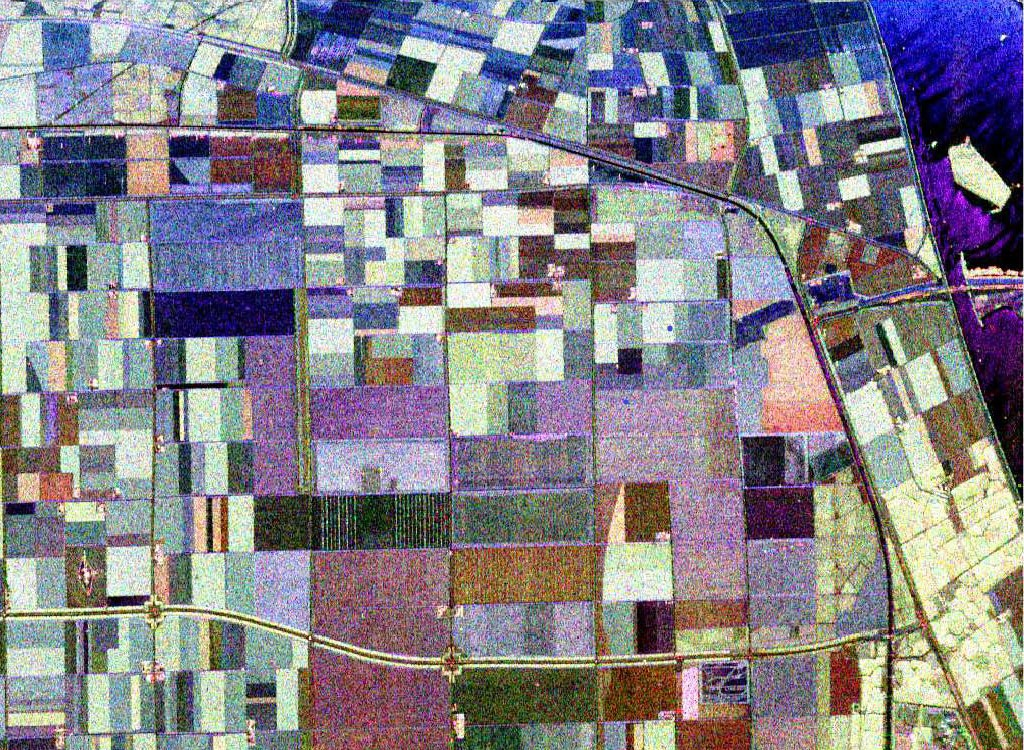
\includegraphics[width=7.04cm]{pic/chapter3/fle/pauli.png}
    }
    \subfloat[]{
        \label{flevoland_gt}
        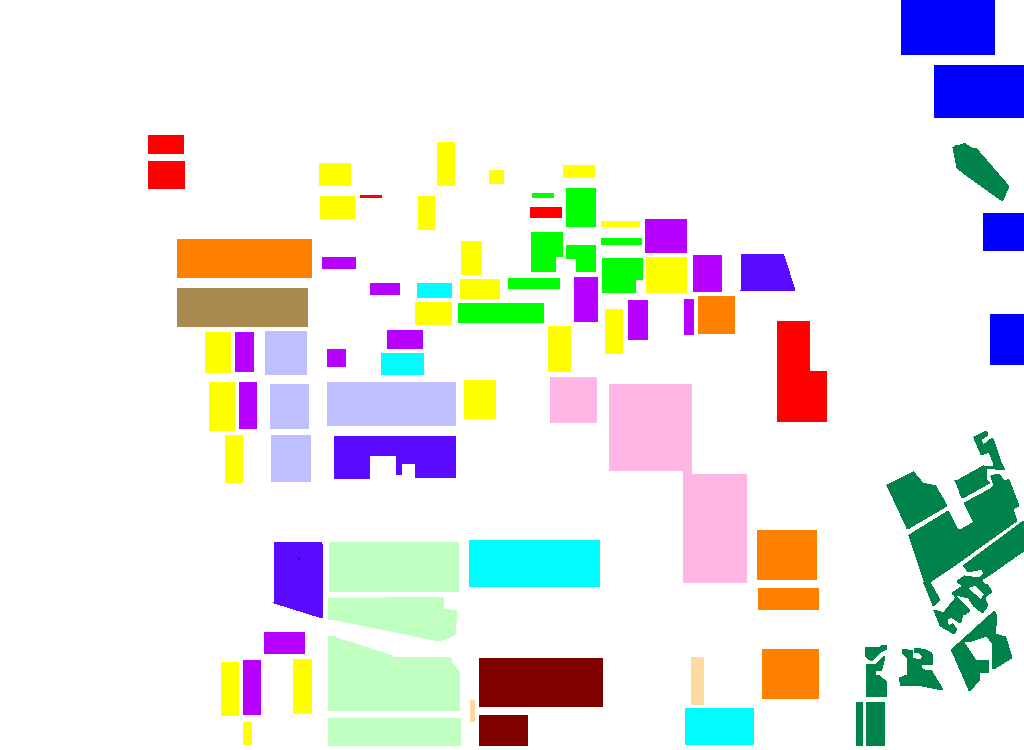
\includegraphics[width=7.04cm]{pic/chapter3/fle/gt.png}
    }

    \subfloat[]{
        \label{pice}
        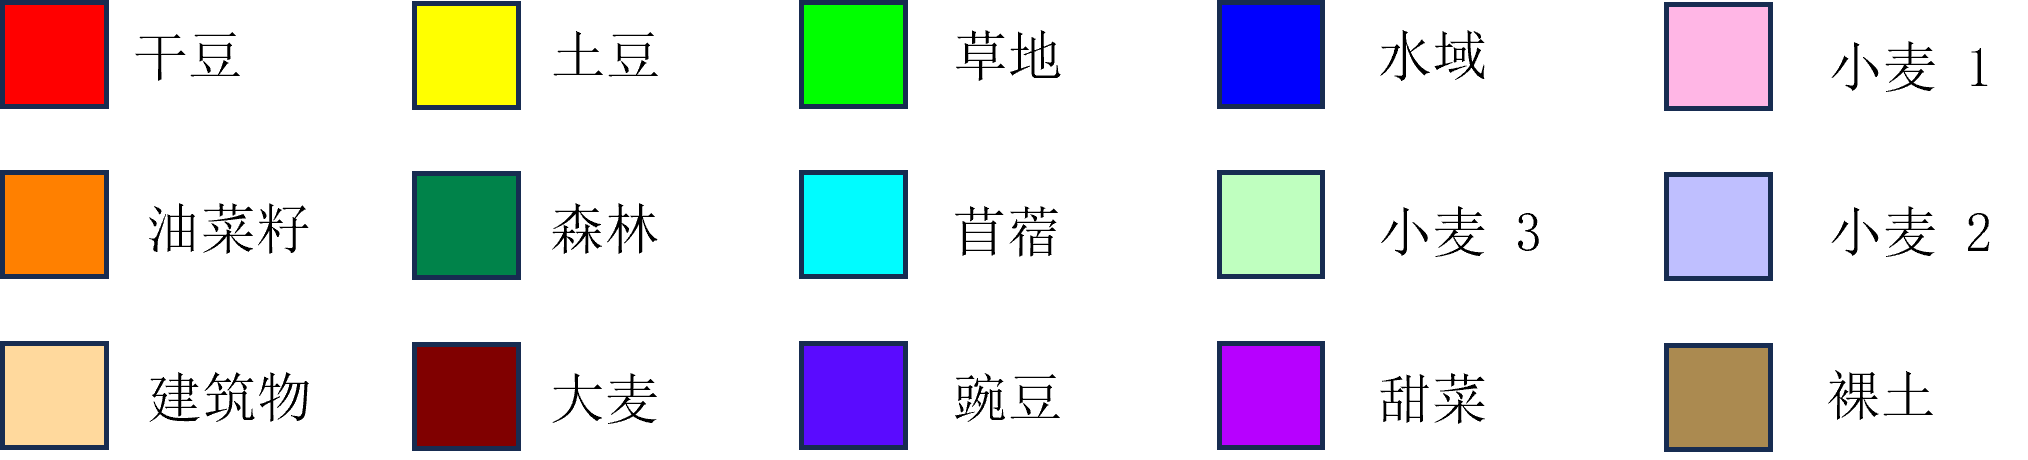
\includegraphics[width=9.04cm]{pic/chapter3/fle/label.png}
    }
    \caption{Flevoland地区实验数据集。(a)Pauli分解伪彩色图像;(b)实验数据地面真值;(c)颜色与类别对应关系}
    \label{fig2}
\end{figure}

\begin{table}[ht!]
    \caption{Felvoand地区实验数据集有标签样本数量}
    \begin{tabular}{|c|c|c|c|c|c|c|c|c|}
        \hline 类别 & 干豆   & 大麦    & 裸土    & 土豆    & 甜菜    & 小麦 1  & 豌豆    & 苜蓿
        \\
        \hline 数目 & 6338 & 7595  & 5109  & 16156 & 10033 & 11159 & 9582  & 10181 \\
        \hline 类别 & 草地   & 小麦 2  & 油菜籽   & 小麦 3  & 建筑物   & 森林    & 水域    &       \\
        \hline 数目 & 7058 & 16386 & 13863 & 22241 & 735   & 18044 & 13232 &       \\
        \hline
    \end{tabular}
    \label{flevoland_smaple}
\end{table}

图\ref{fig:fle_res}展示了各个对比方法的可视化分类结果,其中每个分类结果图下方依次为A、B、C区域的局部放大图。根据图\ref{fig:fle_T},仅使用散射特征的分类方法,在草地(区域A)、油菜籽(区域B)和土豆(区域C)都有较多的错分样本,这是因为只使用了散射特征而忽略了目标分解特征,没有全面综合利用所有的极化信息导致的。图\ref{fig:fle_P}展示了仅使用目标分解特征的分类结果,在草地、油菜籽、土豆区域也存在大量的错分样本,这可能是由于没有综合使用极化信息导致的,相干矩阵代表的散射特征是极化SAR中最基本、重要的特征。图\ref{fig:fle_F}展示的简单叠加散射特征与目标分解特征的分类结果,该方法的分类结果几乎与前两种方法相同,仍然在草地、油菜籽区域存在大量错分样本,这反映了直接简单堆叠使用极化特征带来的准确率提升有限。图\ref{fig:fle_SE}与图\ref{fig:fle_CBAM}展示了使用经典注意力方法的分类结果图,相比于直接叠加特征,并没有带来明显的分类性能提升,少量的错分孤立点与草地中错分的块状区域依然存在,这表明不考虑极化SAR数据特征的特征细化方法并不能为极化SAR分类任务带来优势。图\ref{fig:fle_DP}展示了基于双通道注意力方法的分类结果,可以看出本方法分类结果更加平滑,错分像素减少,特别是是在小麦、油菜籽区域,类间错分孤立点相对减少,这也验证了本章方法结合散射特征和目标分解特征的有效性,证明本章方法提取的极化信息表示是优越的。


% 该方法的分类结果要优于前面两种方法,类间错分孤立点相对减少,具有更少的错分样本,这反映了综合利用极化信息对目标分类具有一定的优势。
\begin{figure}[ht]
    \subfloat[]{
        \label{fig:fle_T}
        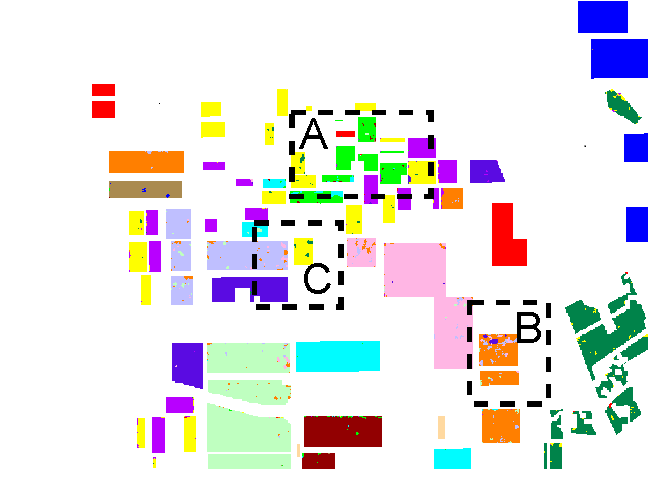
\includegraphics[width=4.74cm]{pic/chapter3/fle/CNN-T.pdf}
    }
    \subfloat[]{
        \label{fig:fle_P}
        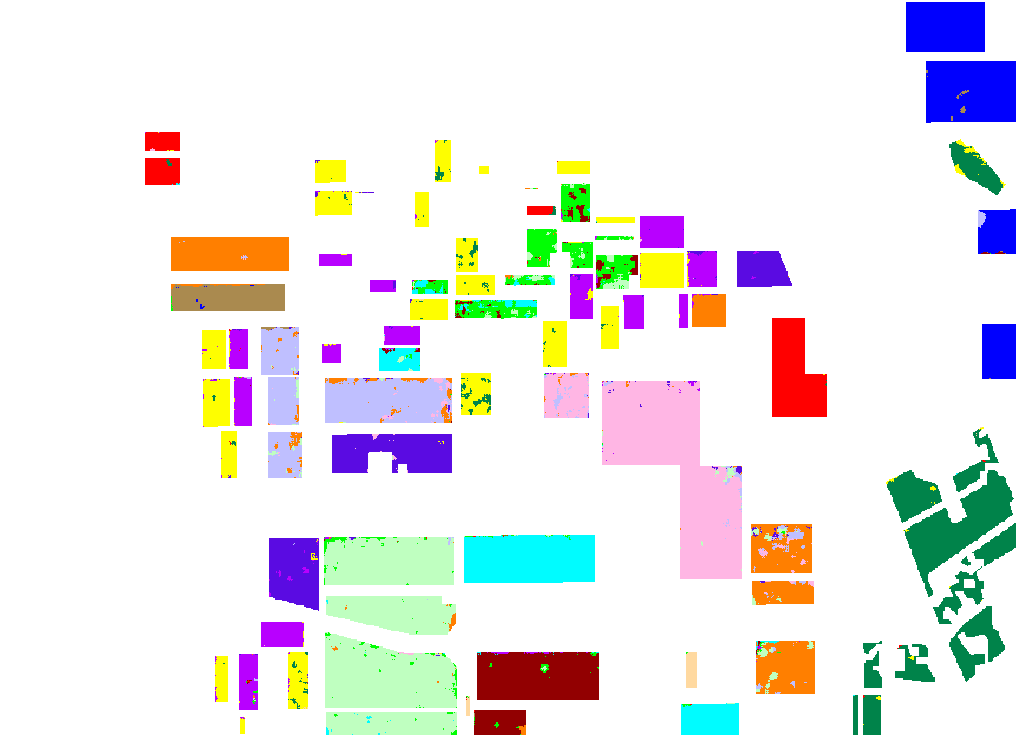
\includegraphics[width=4.74cm]{pic/chapter3/fle/CNN-P.png}
    }
    \subfloat[]{
        \label{fig:fle_F}
        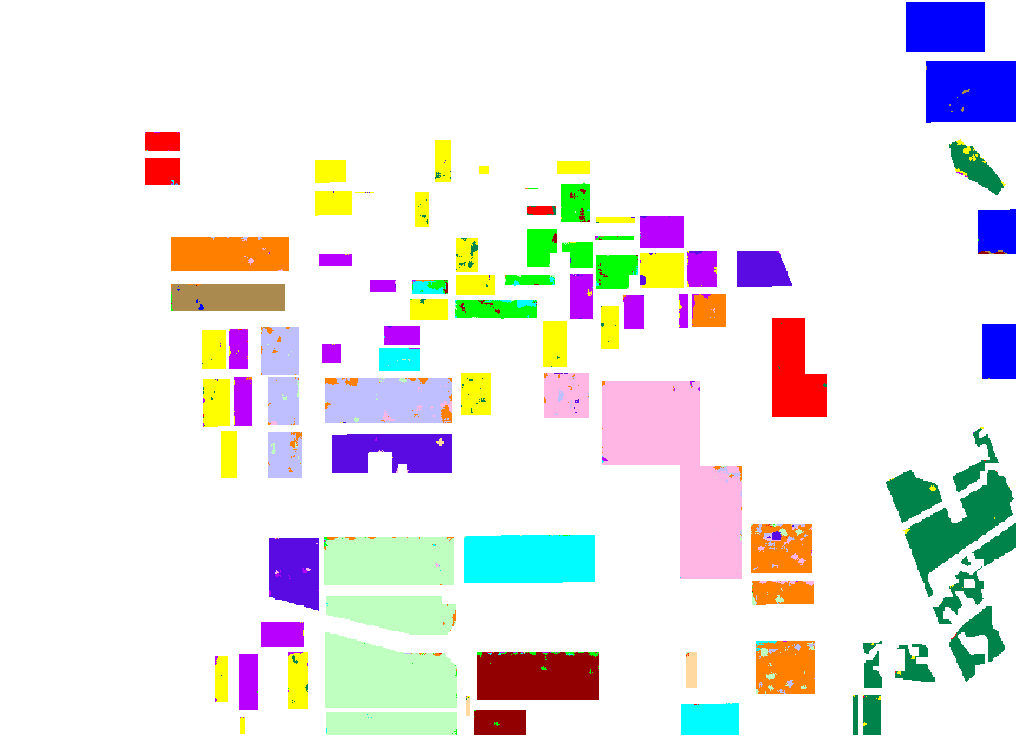
\includegraphics[width=4.74cm]{pic/chapter3/fle/CNN-F.png}
    }

    \begin{minipage}[b]{4.74cm} % 添加minipage环境,4.74cm是子图的宽度
        \subfloat[]{
            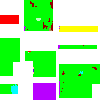
\includegraphics[width=1.4cm]{pic/chapter3/fle/sub-images/0_CNN-T.PNG} % 第一张子图的路径
            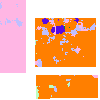
\includegraphics[width=1.4cm]{pic/chapter3/fle/sub-images/1_CNN-T.PNG} % 第二张子图的路径
            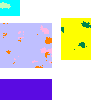
\includegraphics[width=1.4cm]{pic/chapter3/fle/sub-images/2_CNN-T.PNG} % 第三张子图的路径
        }
    \end{minipage}
    \begin{minipage}[b]{4.74cm} % 添加minipage环境,4.74cm是子图的宽度
        \subfloat[]{
            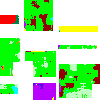
\includegraphics[width=1.4cm]{pic/chapter3/fle/sub-images/0_CNN-P.PNG} % 第一张子图的路径
            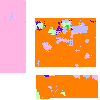
\includegraphics[width=1.4cm]{pic/chapter3/fle/sub-images/1_CNN-P.PNG} % 第二张子图的路径
            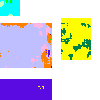
\includegraphics[width=1.4cm]{pic/chapter3/fle/sub-images/2_CNN-P.PNG} % 第三张子图的路径
        }
    \end{minipage}
    \begin{minipage}[b]{4.74cm} % 添加minipage环境,4.74cm是子图的宽度
        \subfloat[]{
            
\includegraphics[width=1.4cm]{pic/chapter3/fle/sub-images/0_CNN-F.PNG} % 第一张子图的路径
            
\includegraphics[width=1.4cm]{pic/chapter3/fle/sub-images/1_CNN-F.PNG} % 第二张子图的路径
            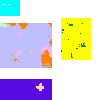
\includegraphics[width=1.4cm]{pic/chapter3/fle/sub-images/2_CNN-F.PNG} % 第三张子图的路径
        }
    \end{minipage}

    \subfloat[]{
        \label{fig:fle_SE}
        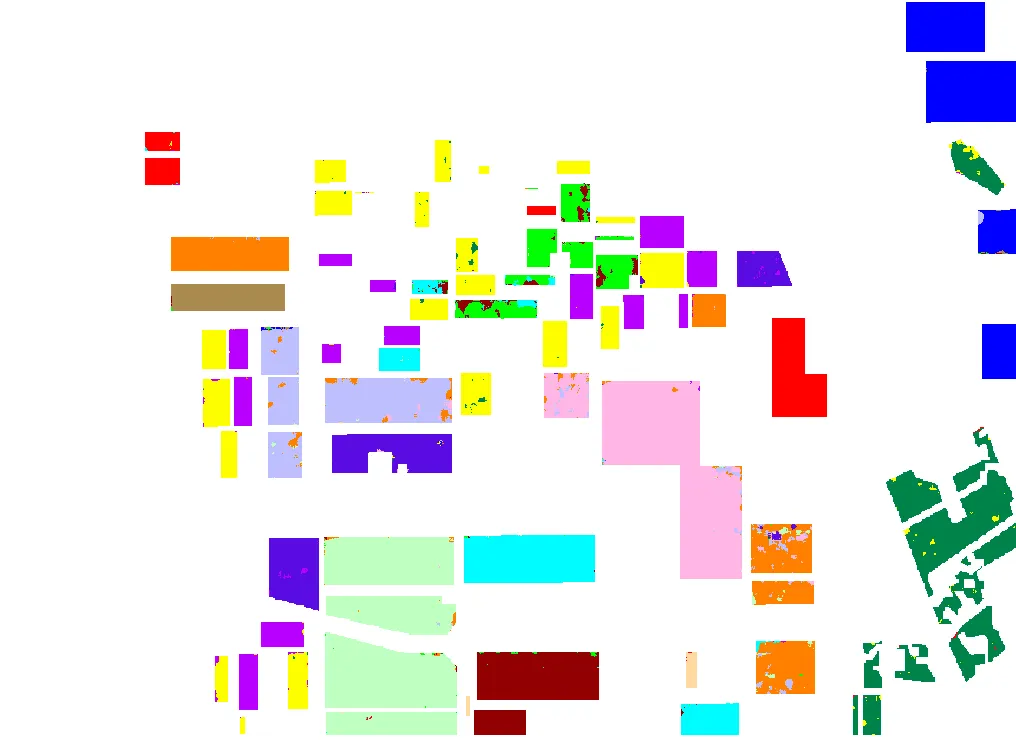
\includegraphics[width=4.74cm]{pic/chapter3/fle/CNN-SE.png}
    }
    \subfloat[]{
        \label{fig:fle_CBAM}
        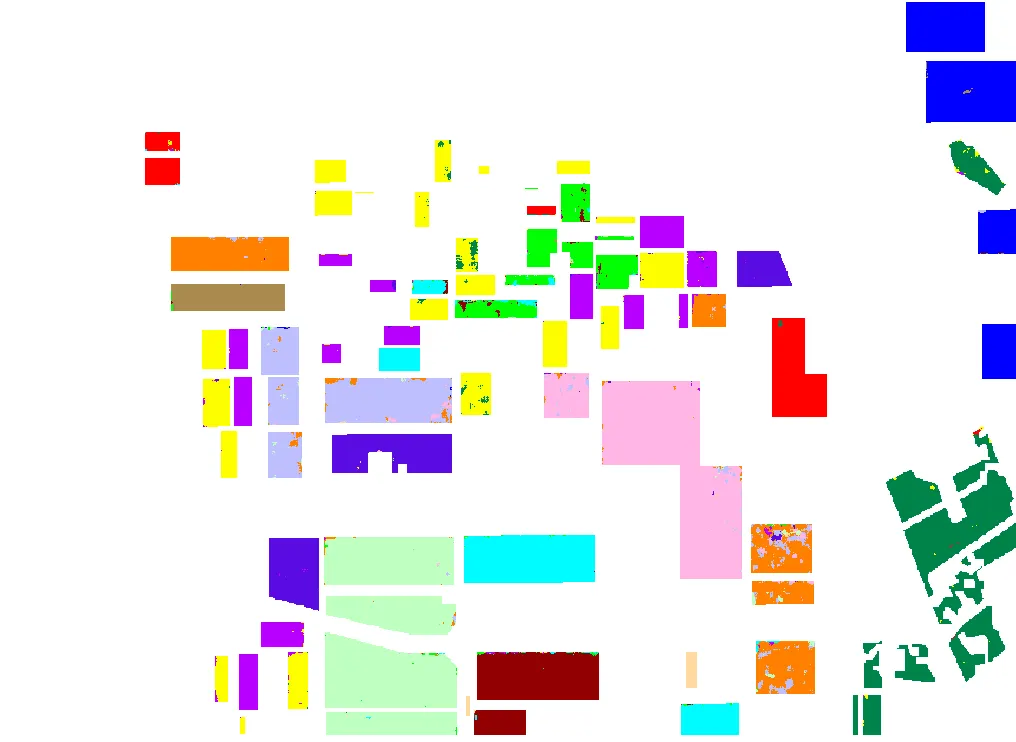
\includegraphics[width=4.74cm]{pic/chapter3/fle/CNN-CBAM.png}
    }
    \subfloat[]{
        \label{fig:fle_DP}
        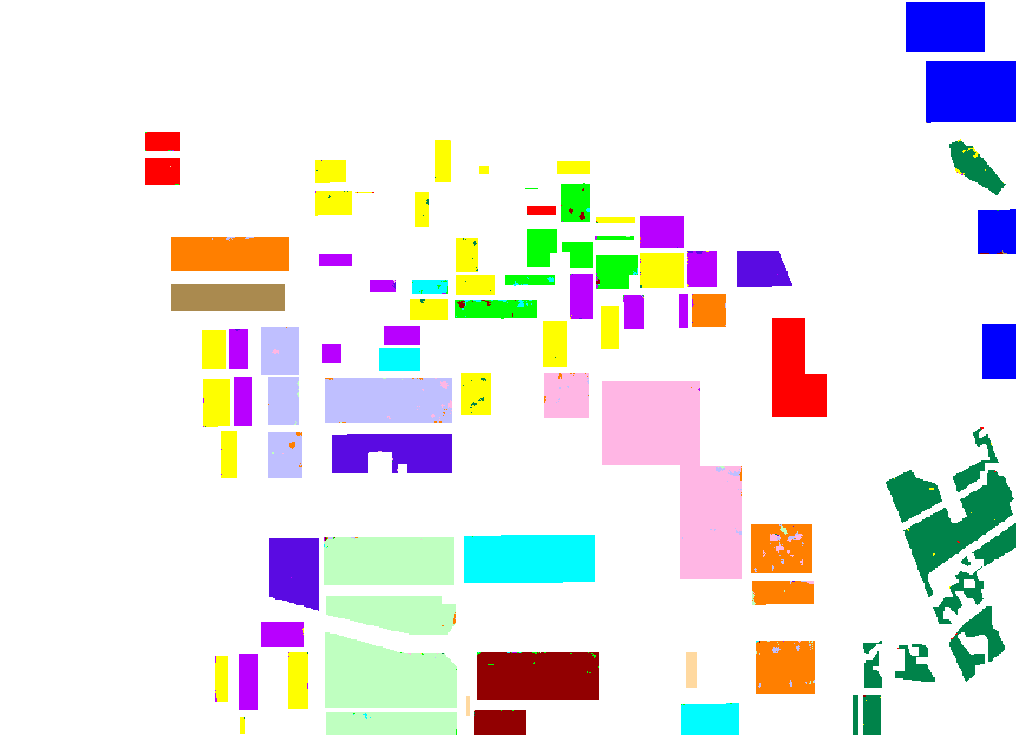
\includegraphics[width=4.74cm]{pic/chapter3/fle/CNN-DP.png}
    }

    \begin{minipage}[b]{4.74cm} % 添加minipage环境,4.74cm是子图的宽度
        \subfloat[]{
            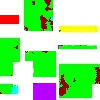
\includegraphics[width=1.4cm]{pic/chapter3/fle/sub-images/0_CNN-SE.PNG} % 第一张子图的路径
            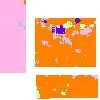
\includegraphics[width=1.4cm]{pic/chapter3/fle/sub-images/1_CNN-SE.PNG} % 第二张子图的路径
            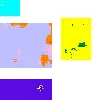
\includegraphics[width=1.4cm]{pic/chapter3/fle/sub-images/2_CNN-SE.PNG} % 第三张子图的路径
        }
    \end{minipage}
    \begin{minipage}[b]{4.74cm} % 添加minipage环境,4.74cm是子图的宽度
        \subfloat[]{
            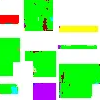
\includegraphics[width=1.4cm]{pic/chapter3/fle/sub-images/0_CNN-CBAM.PNG} % 第一张子图的路径
            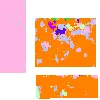
\includegraphics[width=1.4cm]{pic/chapter3/fle/sub-images/1_CNN-CBAM.PNG} % 第二张子图的路径
            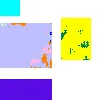
\includegraphics[width=1.4cm]{pic/chapter3/fle/sub-images/2_CNN-CBAM.PNG} % 第三张子图的路径
        }
    \end{minipage}
    \begin{minipage}[b]{4.74cm} % 添加minipage环境,4.74cm是子图的宽度
        \subfloat[]{
            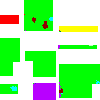
\includegraphics[width=1.4cm]{pic/chapter3/fle/sub-images/0_CNN-DP.PNG} % 第一张子图的路径
            
\includegraphics[width=1.4cm]{pic/chapter3/fle/sub-images/1_CNN-DP.PNG} % 第二张子图的路径
            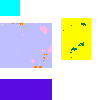
\includegraphics[width=1.4cm]{pic/chapter3/fle/sub-images/2_CNN-DP.PNG} % 第三张子图的路径
        }
    \end{minipage}
    \caption{AIRSAR Flevoland地区数据分类可视化结果图。(a)CNN-T;(b)CNN-P;(c)CNN-F;(d)CNN-T局部误差图;(e)CNN-P局部误差图;(f)CNN-F局部误差图;(g)CNN-SE;(h)CNN-CBAM;(i)本章方法;(j)CNN-SE局部误差图;(h)CNN-CBAM局部误差图;(i)本章方法局部误差图}
    \label{fig:fle_res}
\end{figure}

为了进一步探索极化信息提取模块的性能,引入t-SNE(t-distributed Stochastic Neighbor Embedding)\citing{van2008visualizing}特征分布图作为衡量极化信息提取模块的可视化评估指标。t-SNE是一种非线性降维技术,能够有效地将高维数据映射到二维或三维空间,以便更直观地观察样本在特征空间的分布。

图\ref{fig:fle-tSNE}展示了不同方法特征特征使用t-SNE可视化的分布情况。根据图\ref{fig:fle_t_t}、图\ref{fig:fle_t_p}和图\ref{fig:fle_t_f}所展示的仅散射特征、仅分解特征和直接堆叠特征三种不同的特征分布情况,可以看出大多数类别相互之间有交叠的情况,并且类内的样本分布较为散乱,因而容易造成类间错分的情况,导致分类性能优先。而图\ref{fig:fle_t_se}和图\ref{fig:fle_t_cbam}展示的使用经典的注意力信息提取方法的特征分布图,可以看出经典的注意力方法由于没有考虑极化SAR的数据特性,不同类别之间的重叠情况依然存在,并且类内样本特征分布散乱,证明了在信息提取时不考虑极化SAR数据特征对分类模型的性能提升是有限的。根据图\ref{fig:fle_t_dp}所展示的基于双通道注意力的极化信息提取方法的特征分布图,可以看到相比于其他的特征分布情况,类间的交叠现象有了明显的改善,同时类内样本特征分布更加紧凑,提升类间可分性,进而带来分类性能上的提升。


\begin{figure}[ht]
    \subfloat[]{
        \label{fig:fle_t_t}
        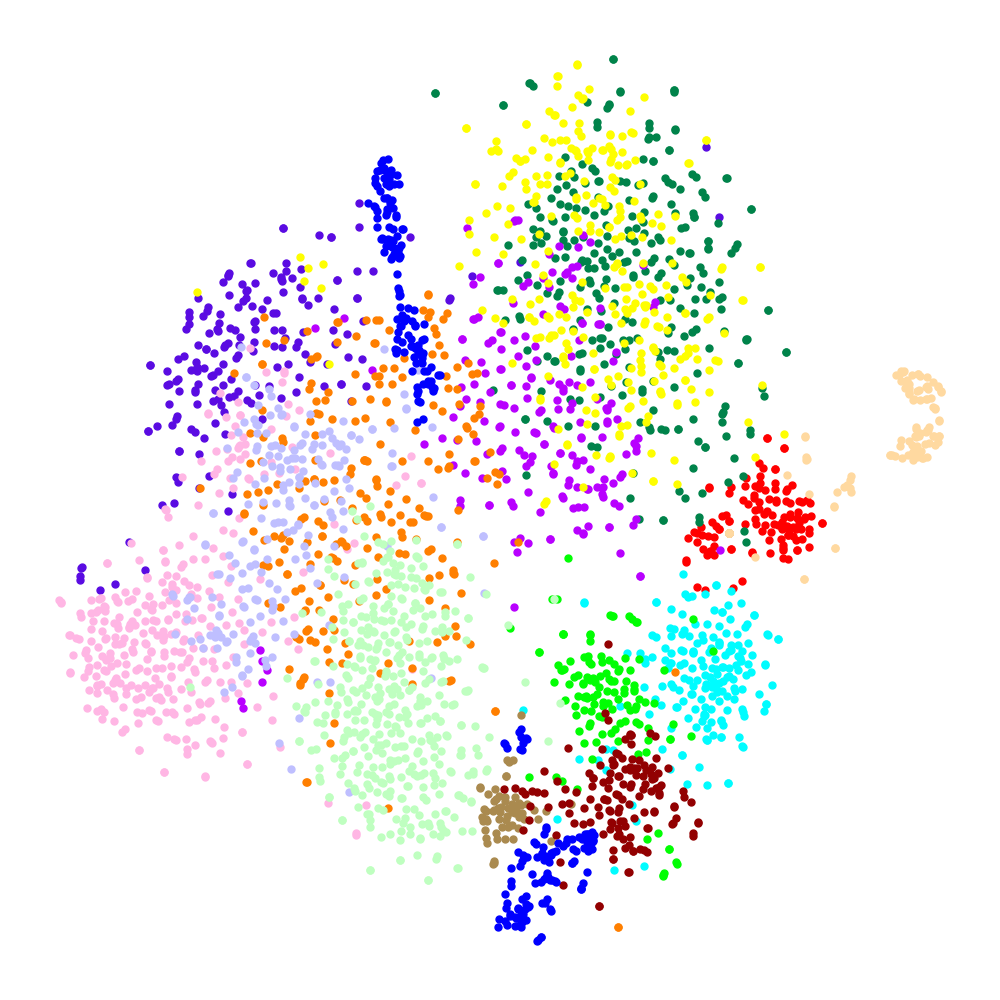
\includegraphics[width=4.74cm]{pic/chapter3/fle/t-sne/t.png}
    }
    \subfloat[]{
        \label{fig:fle_t_p}
        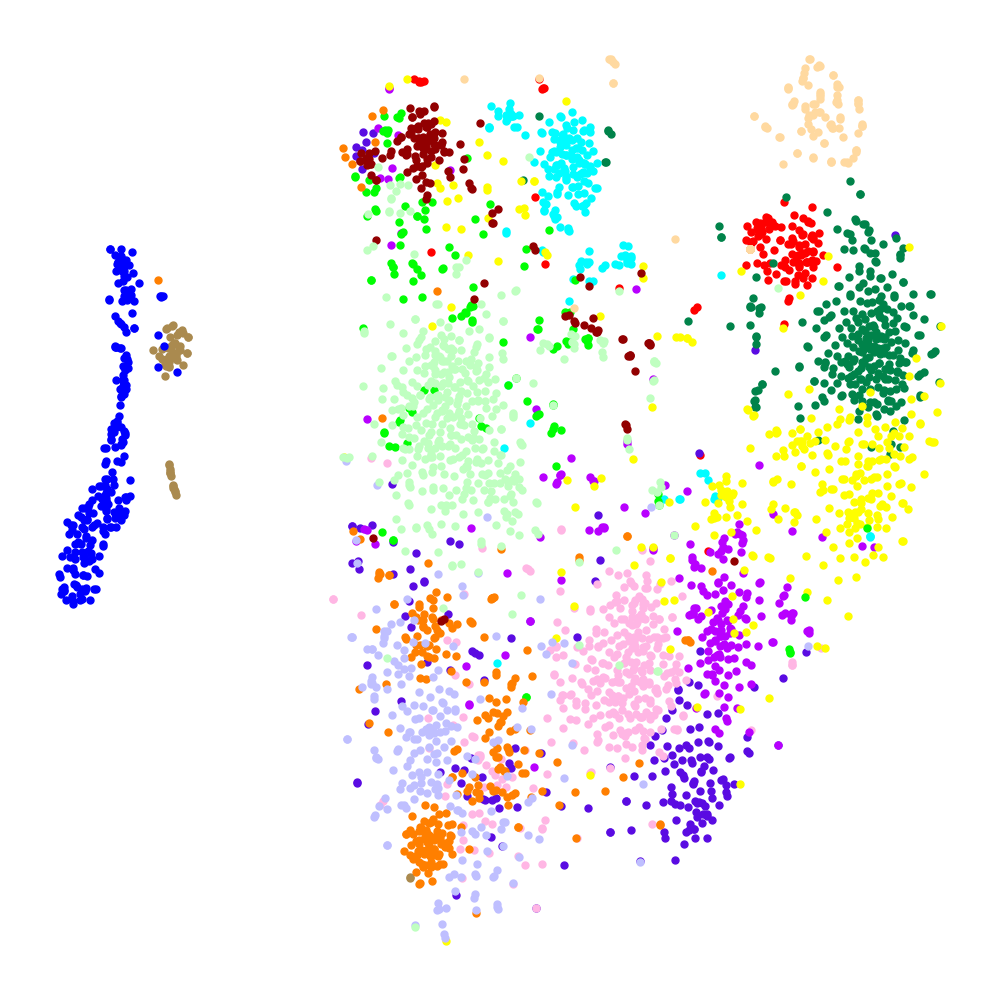
\includegraphics[width=4.74cm]{pic/chapter3/fle/t-sne/p.png}
    }
    \subfloat[]{
        \label{fig:fle_t_f}
        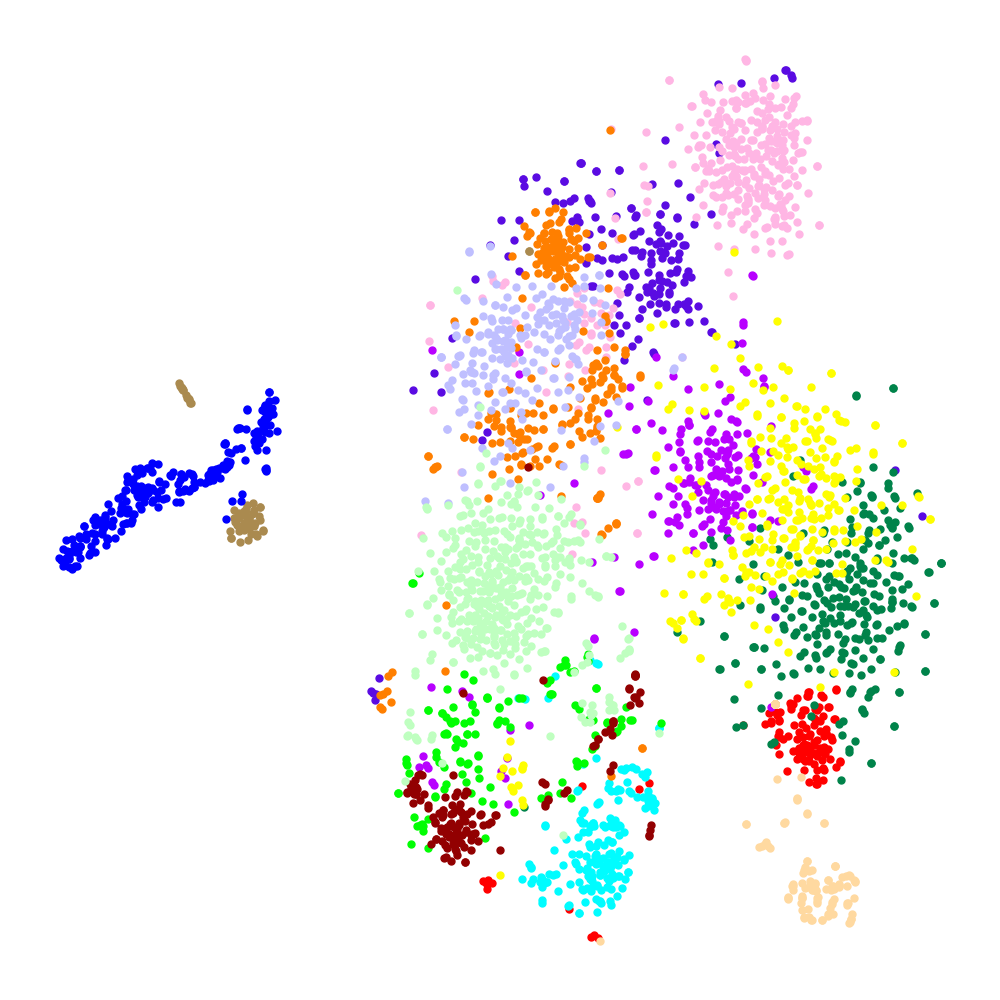
\includegraphics[width=4.74cm]{pic/chapter3/fle/t-sne/f.png}
    }

    \subfloat[]{
        \label{fig:fle_t_se}
        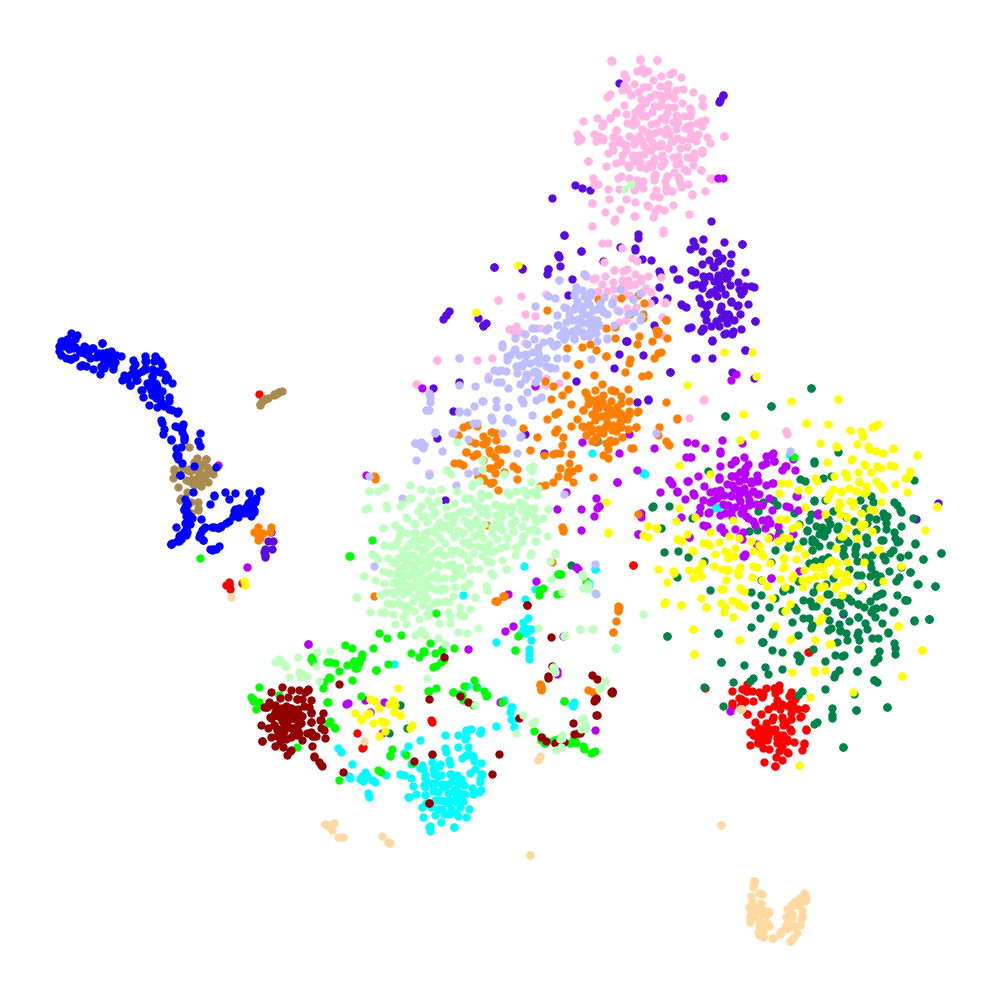
\includegraphics[width=4.74cm]{pic/chapter3/fle/t-sne/se.png}
    }
    \subfloat[]{
        \label{fig:fle_t_cbam}
        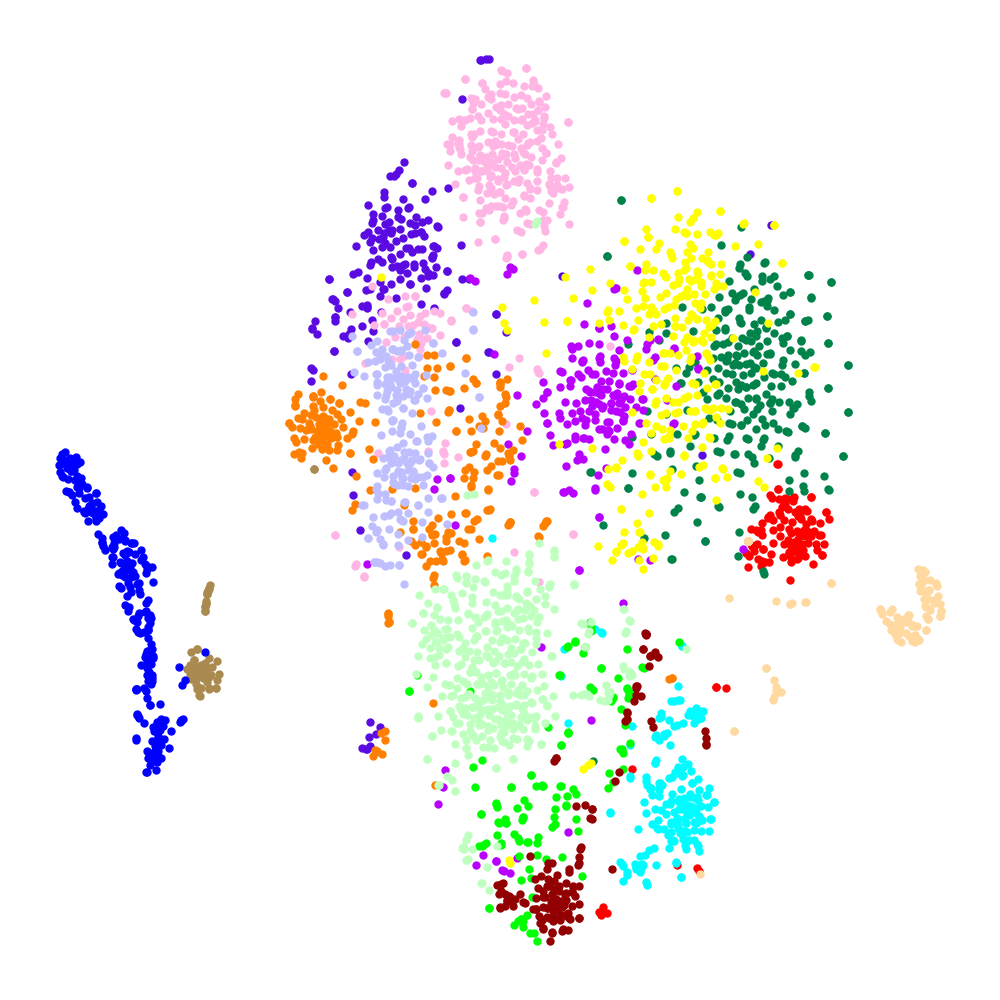
\includegraphics[width=4.74cm]{pic/chapter3/fle/t-sne/cbam.png}
    }
    \subfloat[]{
        \label{fig:fle_t_dp}
        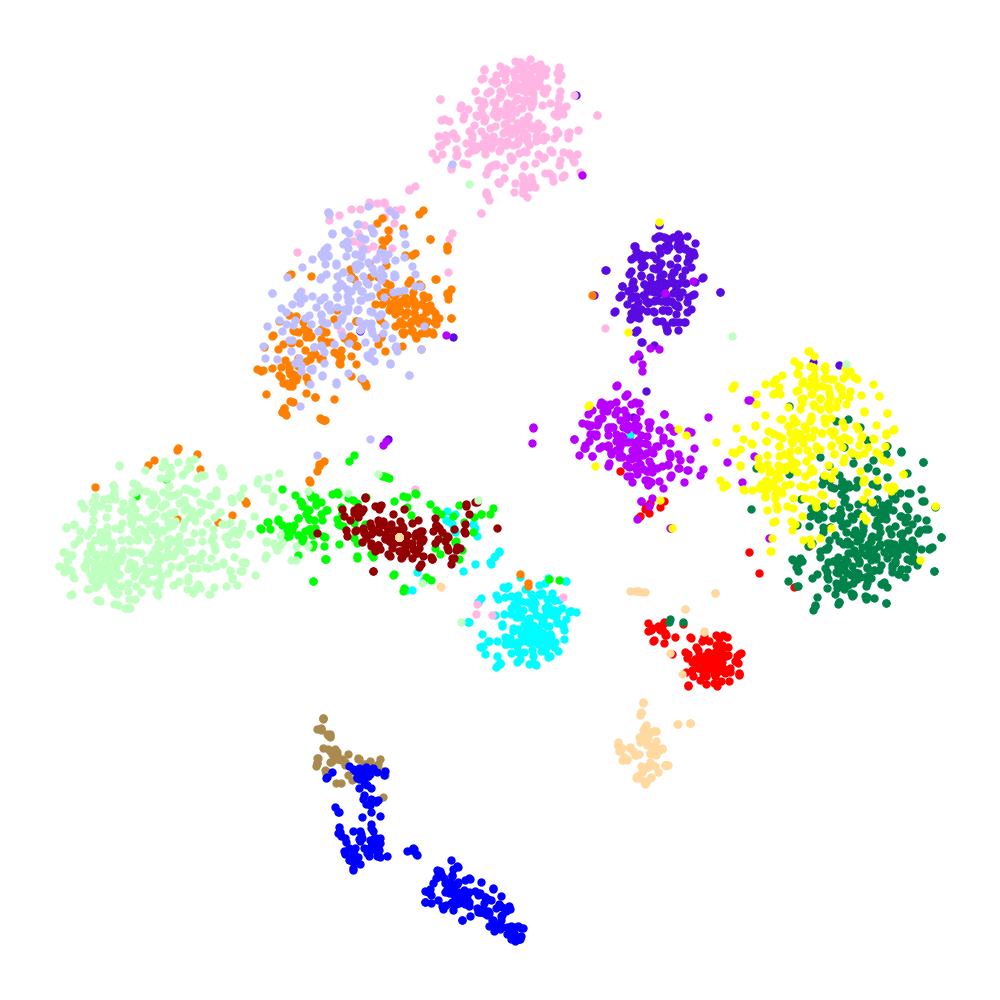
\includegraphics[width=4.74cm]{pic/chapter3/fle/t-sne/dp.png}
    }

    \subfloat[]{
        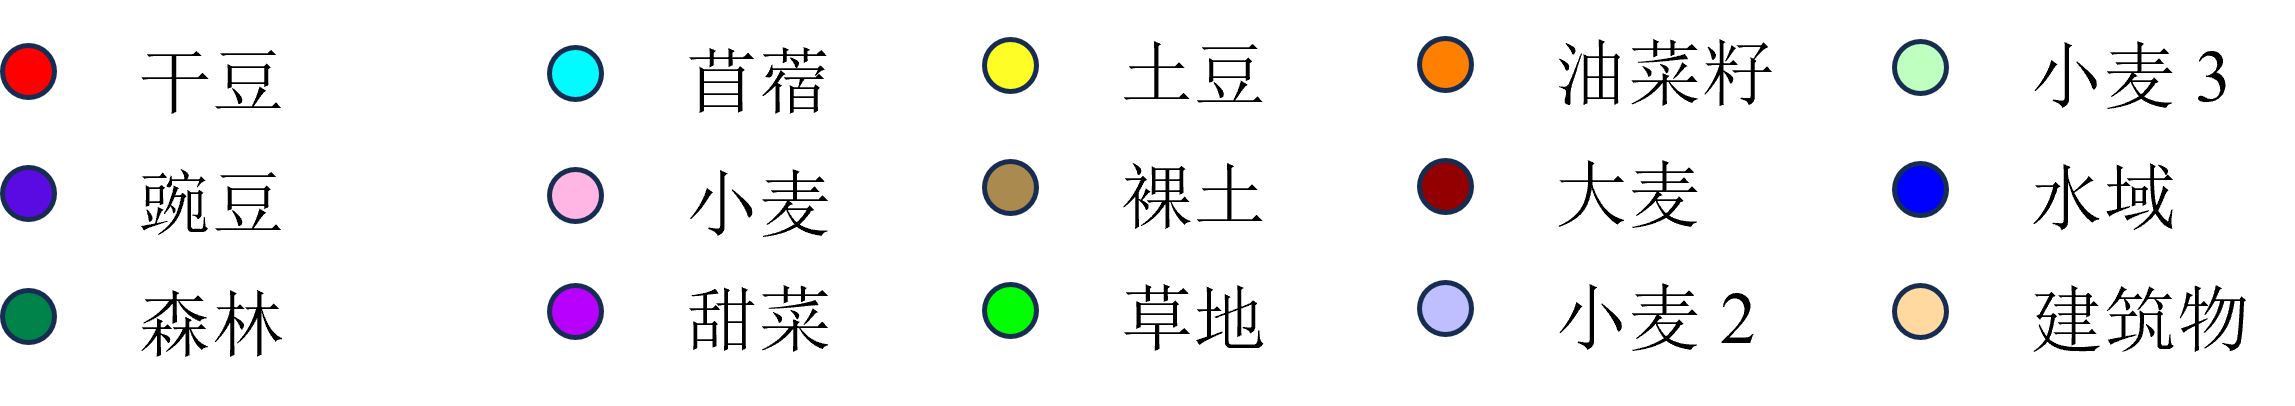
\includegraphics[width=10.04cm]{pic/chapter3/fle/tSNE-label.png}
    }
    \caption{AIRSAR Flevoland地区数据不同方法特征分布。(a)CNN-T;(b)CNN-P;(c)CNN-F;(d)CNN-SE;(e)CNN-CBAM;(f)本章方法;(g)颜色与类别对应关系}
    \label{fig:fle-tSNE}
\end{figure}

表\ref{tab:fle_result}展示了不同方法的分类数值结果。仅使用散射特征的分类方法,在草地和建筑物区域的分类准确率较低,分别为89.41\%和91.17\%,这可能是因为仅使用相干矩阵作为极化特征的分类方法,并不能完全反应这两类地物目标的散射特性,导致分类准确率较低。仅使用目标分解特征作为特征的分类方法,在干豆区域达到了99.66\%的准确率,这是因为目标分解特征中包含有具体物理意义的极化表征,但是在建筑物油菜籽区域的分类准确率较低,仅有90.2\%,反映了目标分解特征与散射特征相互补充,都是必不可少的极化特征表示方法。直接堆叠极化特征的分类方法在分类总体准确率、平均准确率以及大麦等区域准确率反而下降,这表明了直接堆叠极化特征导致特征维数增加,分类器无法有效分清两种类型的主次关系,导致分类准确率有所下降。经典的注意力方法CNN-SE与CNN-CBAM的OA指标分别为96.76\%和96.13\%,相比于前面的方法仅有不足1\%的提升,表明该方法直接应用于极化SAR领域性能提升有限。而本章方法在大多数的类别都具有最高的分类准确率,OA、AA与Kappa分别达到98.47\%、98.65\%和98.53\%,相比于其他方法分别提升了1.71\%、3.12\%和2.46\%,表明了基于双通道注意力的极化信息提取方法对于极化SAR目标分类具有优势,验证了本章方法的有效性与优越性。

\begin{table}[ht!]
    \caption{AIRSAR Flevoland地区数据分类数值结果(\%)}
    \label{tab:fle_result}
    \renewcommand\arraystretch{1.0}
    \begin{tabular}{cccccccc}
        \toprule[1.5bp]
        序号                        & 类别    & CNN-T & CNN-P          & CNN-F & CNN-SE         & CNN-CBAM       & CNN-DP         \\
        \midrule[0.75bp]
        1                         & 建筑物   & 91.17 & 90.2           & 94.01 & \textbf{99.79} & 94.14          & 98.83          \\
        2                         & 油菜籽   & 94.33 & 91.78          & 89.78 & 94.54          & 92.32          & \textbf{98.29} \\
        3                         & 甜菜    & 96.57 & 96.62          & 96.99 & 97.92          & 95.74          & \textbf{98.92} \\
        4                         & 干豆    & 99.26 & \textbf{99.66} & 98.86 & 97.08          & 98.83          & 99.58          \\
        5                         & 豌豆    & 96.72 & 97.03          & 96.54 & 99.8           & 95.72          & \textbf{99.25} \\
        6                         & 森林    & 98.13 & 97.37          & 96.42 & 98.85          & 98.61          & \textbf{99.08} \\
        7                         & 苜蓿    & 96.03 & 95.96          & 95.07 & 96.11          & 95.48          & \textbf{97.86} \\
        8                         & 土豆    & 96.61 & 97.03          & 97.54 & 97.33          & 95.59          & \textbf{99}    \\
        9                         & 裸土    & 95.02 & 97.19          & 98.44 & 98.51          & 96.8           & \textbf{99.67} \\
        10                        & 草地    & 89.41 & 93.11          & 92.32 & 96.19          & 94.25          & \textbf{97.81} \\
        11                        & 大麦    & 93.63 & 95.45          & 87.34 & 95.64          & 89.34          & \textbf{97.7}  \\
        12                        & 水域    & 99.94 & 99.7           & 99.66 & 93.3           & 99.83          & \textbf{99.99} \\
        13                        & 小麦 1  & 97.53 & 96.74          & 97.36 & 97.27          & 97.6           & \textbf{97.92} \\
        14                        & 小麦 2  & 93.62 & 94.48          & 94.21 & \textbf{97.53} & 92.25          & 96.53          \\
        15                        & 小麦 3  & 96.88 & 97.05          & 98.06 & 94.85          & 98.51          & \textbf{99.36} \\
        \midrule[0.75bp]
        \multicolumn{2}{c}{OA}    & 96.4  & 96.41 & 95.9           & 96.76 & 96.13          & \textbf{98.47}                  \\
        \multicolumn{2}{c}{AA}    & 95.68 & 95.93 & 95.51          & 96.98 & 95.67          & \textbf{98.65}                  \\
        \multicolumn{2}{c}{Kappa} & 96.07 & 96.08 & 95.53          & 96.48 & 95.77          & \textbf{98.53}                  \\
        \bottomrule[1.5bp]
    \end{tabular}
\end{table}

图\ref{fig:fle_conf_matrix}展示了本章方法分类结果对应的混淆矩阵。结果表明,混淆矩阵的主对角线元素具有相对较高的数值,模型正确分类的情况占据了主导地位,说明本章方法在本数据集上的优秀分类性能。

\begin{figure}[h]
    \centering
    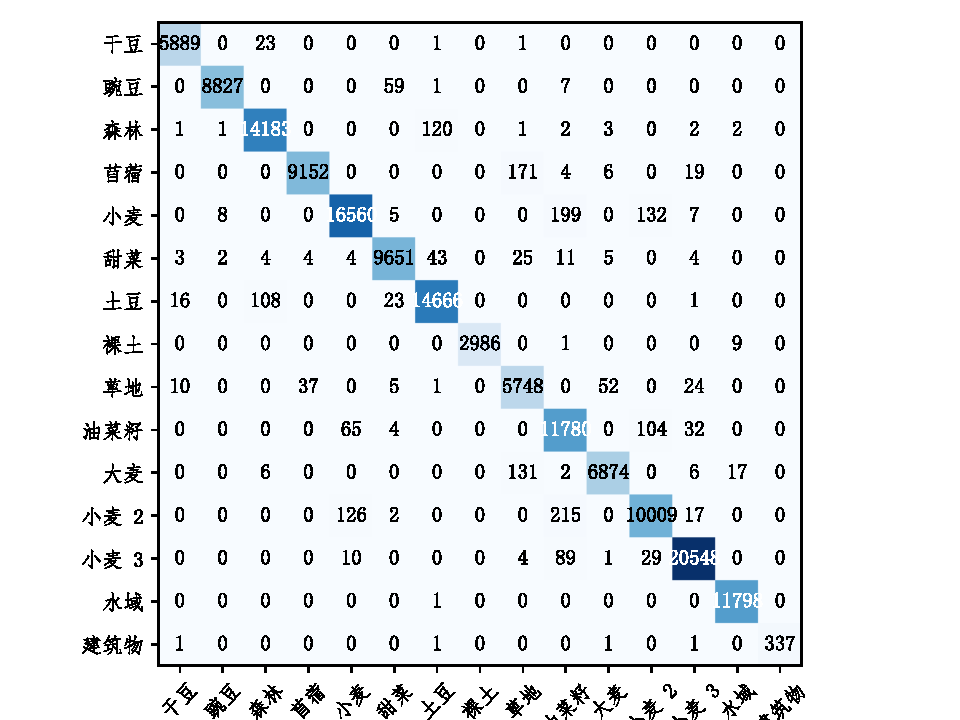
\includegraphics[width=10.4cm]{pic/chapter3/fle/conf-matrix.pdf}
    \caption{本章方法在Flevoland图像中分类结果混淆矩阵图}
    \label{fig:fle_conf_matrix}
\end{figure}


\subsection{E-SAR Oberpfaffenhofen数据实验}
该数据集是通过E-SAR机载平台在德国Oberpfaffenhofen地区拍摄获取到的L波段极化SAR数据。该数据集经过多视处理,具有高质量的全极化信息,是极化SAR目标分类研究的经典数据集之一。数据集在方位向和距离向具有$3m \times 3m$的分辨率,大小为$1300 \times 1200$,包含建筑物、林地、开放区域三种类型的地物目标,每类包含样本数量依次为269184、388503、779962。图\ref{fig:ober_pauli}展示了该数据集的Pauli伪彩色图像,图\ref{fig:ober_gt}展示了该数据集的人工标记的地面真值参考图,地面真值图中黑色的区域表示未标记的区域。

\begin{figure}[ht]
    \subfloat[]{
        \label{fig:ober_pauli}
        \includegraphics[width=4.04cm]{pic/chapter3/ober/Pauli.png}
    }
    \subfloat[]{
        \label{fig:ober_gt}
        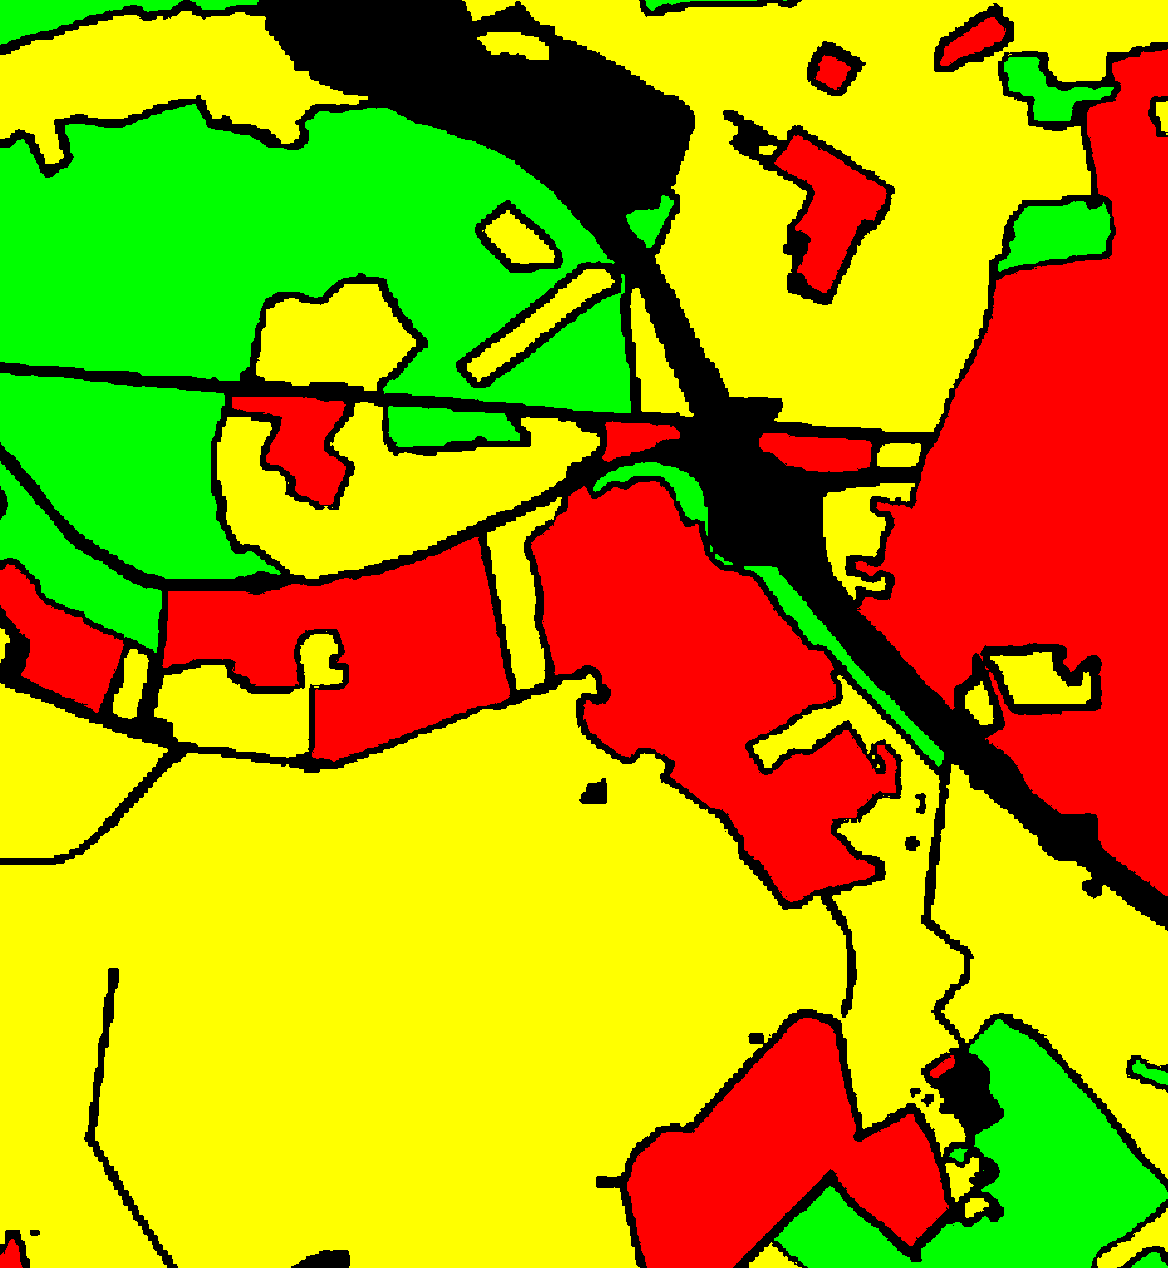
\includegraphics[width=4.04cm]{pic/chapter3/ober/gt.png}
    }

    \subfloat[]{
        \label{fig:ober_label}
        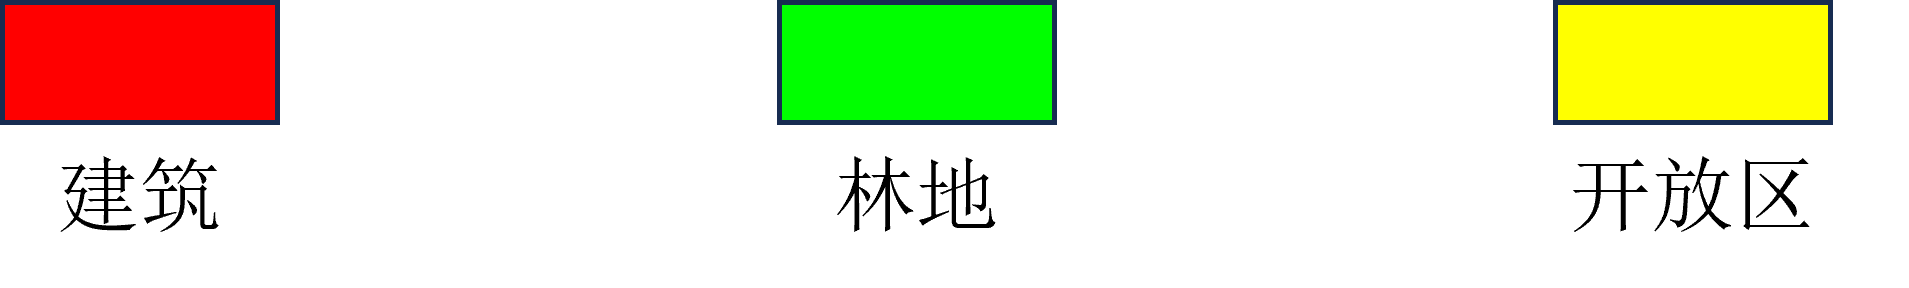
\includegraphics[width=7.04cm]{pic/chapter3/ober/label.png}
    }
    \caption{E-SAR Oberpfaffenhofen区域数据。(a)Pauli分解伪彩色图像;(b)实验数据地面真值;(c)颜色与类别对应关系}
\end{figure}

图\ref{fig:ober_res}展示了不同方法的分类结果可视化图像。根据图\ref{fig:ober_T}展示的仅使用极化相干矩阵为特征的分类结果图,尽管在开放区域的分类效果较好,但是在建筑物(区域A、区域B、区域C)存在大量被错分的样本,将建筑物区域样本错误分类为开放区域,并且错分的现象较为严重。这可能是因为仅使用极化相干矩阵作为特征时并没有完全利用其他的目标分解特征导致的,说明了综合考虑极化SAR图像中的其他极化特性和辅助特征的在分类任务中的重要性。相比之下,图\ref{fig:ober_P}与图\ref{fig:ober_F}在建筑物区域中的错分样本相对较少,但是在各类区域中也存在着部分错分的样本。其中将开放区域中的少数像素分类为建筑物的错分情况依然存在,这反映了极化目标分解特征提供的反映目标物理散射特性的信息为分类任务带来了一定的优势,是极化SAR图像中的重要的基本特征。图\ref{fig:ober_SE}和图\ref{fig:ober_CBAM}展示了基于经典注意力方法的特征表示分类结果,从结果图中可以看出,分类效果仅有微小的变化,错分像素相对减少但是依然存在,这可能是极化SAR图像与光学图像存在较大的差异,经典的注意力方法并没有考虑极化SAR图像的数据特征特点。图\ref{fig:ober_DP}展示了基于本章提出的双通道注意力极化信息提取方法的分类结果图,从图中可以看出,在建筑物区域的错分样本明显减少区域内部分类更加平滑,并且每个类中的小块错误区域数量也相对减少,整体分类结果得到明显改善,证明了本章方法的有效性。

\begin{figure}[ht!]
    \subfloat[]{
        \label{fig:ober_T}
        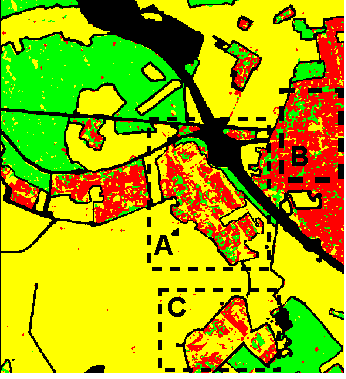
\includegraphics[width=4.04cm]{pic/chapter3/ober/CNN-T.pdf}
    }
    \subfloat[]{
        \label{fig:ober_P}
        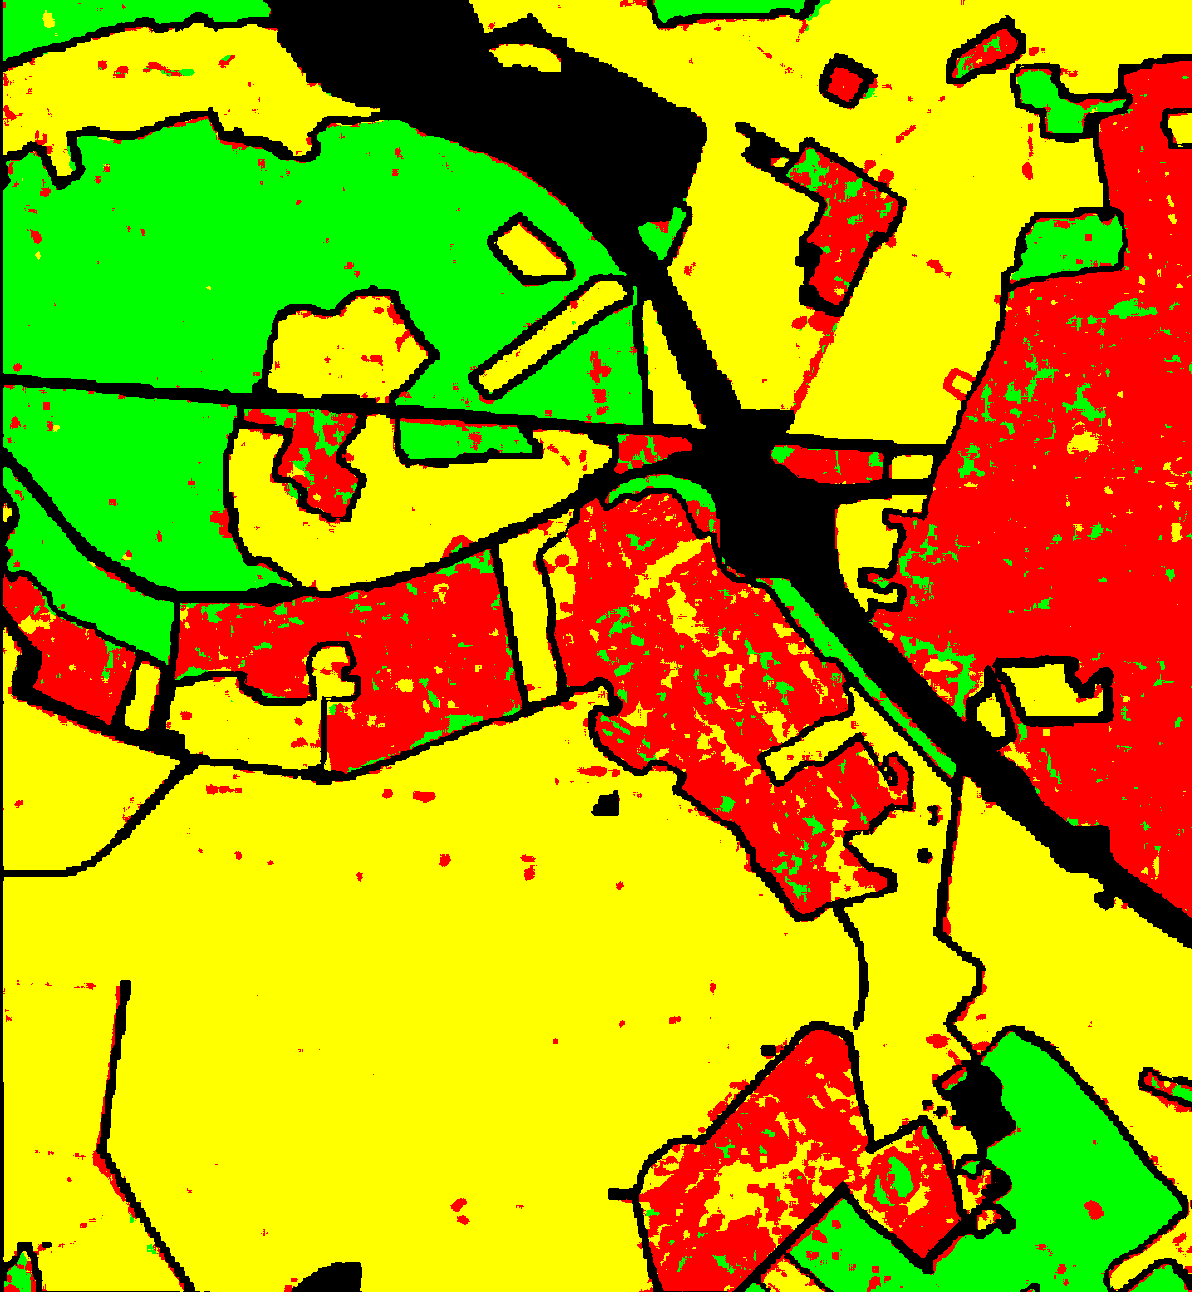
\includegraphics[width=4.04cm]{pic/chapter3/ober/CNN-P.png}
    }
    \subfloat[]{
        \label{fig:ober_F}
        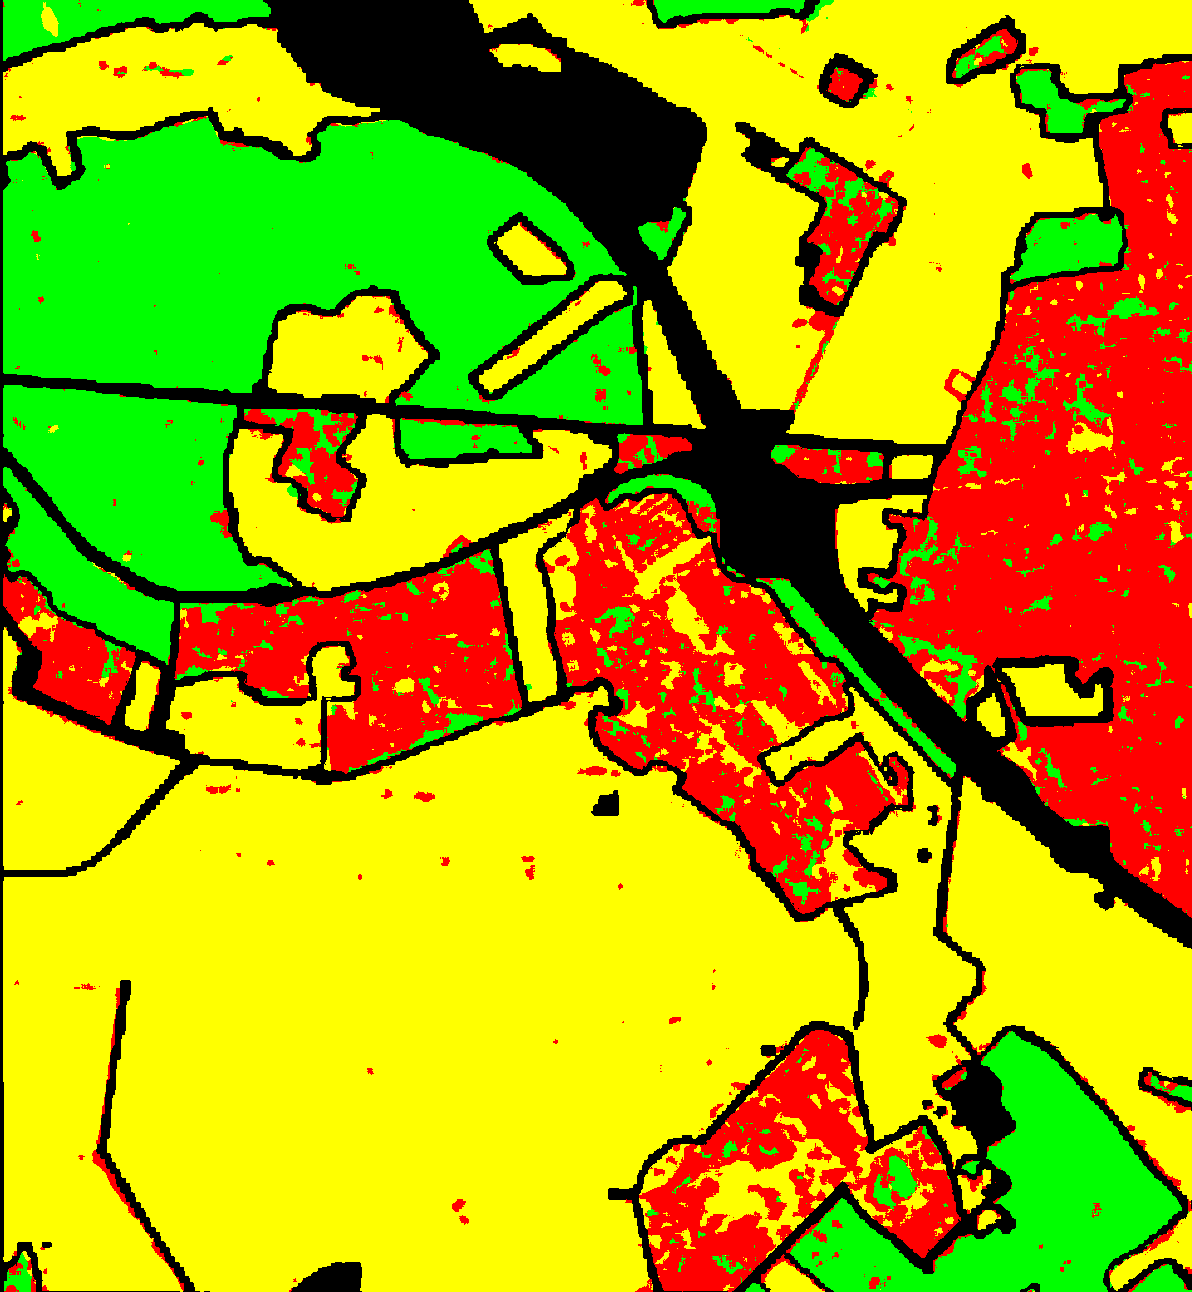
\includegraphics[width=4.04cm]{pic/chapter3/ober/CNN-F.png}
    }

    \subfloat[]{
        \label{fig:ober_SE}
        \includegraphics[width=4.04cm]{pic/chapter3/ober/CNN-SE.png}
    }
    \subfloat[]{
        \label{fig:ober_CBAM}
        \includegraphics[width=4.04cm]{pic/chapter3/ober/CNN-CBAM.png}
    }
    \subfloat[]{
        \label{fig:ober_DP}
        \includegraphics[width=4.04cm]{pic/chapter3/ober/CNN-DP.png}
    }

    \caption{E-SAR Oberpfaffenhofen地区数据分类可视化结果图。(a)CNN-T;(b)CNN-P;(c)CNN-F;(d)CNN-SE;(e)CNN-CBAM;(f)本章方法}
    \label{fig:ober_res}
\end{figure}

图\ref{fig:ober-tSNE}展示了不同方法数据特征使用tSNE可视化的分布情况。根据图\ref{fig:ober_t_t}、图\ref{fig:ober_t_p}、图\ref{fig:ober_t_f}展示的仅散射特征、仅分解特征和直接堆叠的三种特征分布情况,可以看出三种特征分布情况并没有本质性的差异,尽管都可以看出各类之间存在不同的分布情况,但是也能清晰看出,类间存在分布交叠的部分,这也导致了部分样本的错分情况。根据图\ref{fig:ober_t_se}和图\ref{fig:ober_t_cbam}展示的使用经典注意力信息提取方法的特征分布图,可以看出虽然类间交叠的情况有细微改善,但是依然有大量的特征存在交叠,这也映照了分类结果改善不大的结果。图\ref{fig:ober_t_dp}展示了使用本章方法的特征分布情况,可以看出类间交叠的情况得到优化,各类之间分布间距增大,增强了类间可分性,进而带来分类性能的提升。

\begin{figure}[ht!]
    \subfloat[]{
        \label{fig:ober_t_t}
        \includegraphics[width=4.04cm]{pic/chapter3/ober/tSNE-T.png}
    }
    \subfloat[]{
        \label{fig:ober_t_p}
        \includegraphics[width=4.04cm]{pic/chapter3/ober/tSNE-P.png}
    }
    \subfloat[]{
        \label{fig:ober_t_f}
        \includegraphics[width=4.04cm]{pic/chapter3/ober/tSNE-F.png}
    }

    \subfloat[]{
        \label{fig:ober_t_se}
        \includegraphics[width=4.04cm]{pic/chapter3/ober/tSNE-SE.png}
    }
    \subfloat[]{
        \label{fig:ober_t_cbam}
        \includegraphics[width=4.04cm]{pic/chapter3/ober/tSNE-CBAM.png}
    }
    \subfloat[]{
        \label{fig:ober_t_dp}
        \includegraphics[width=4.04cm]{pic/chapter3/ober/tSNE-DP.png}
    }

    \subfloat[]{
        \includegraphics[width=7.04cm]{pic/chapter3/ober/tSNE-label.png}
    }
    \caption{E-SAR Oberpfaffenhofen地区数据地区数据不同方法特征分布。(a) CNN-T; (b) CNN-P; (c) CNN-F; (d) CNN-SE; (e) CNN-CBAM; (f) 本章方法}
    \label{fig:ober-tSNE}
\end{figure}

\begin{table}[ht!]
    \caption{E-SAR Oberpfaffenhofen地区数据分类数值结果(\%)}
    \label{tab:ober_res}
    \begin{tabular}{cccccccc}
        \toprule[1.5bp]
        序号                        & 类别    & CNN-T & CNN-P & CNN-F & CNN-SE & CNN-CBAM       & 本章方法           \\
        \midrule[0.75bp]
        1                         & 建筑    & 76.68 & 83.9  & 80.1  & 80.42  & 83.92          & \textbf{90.47} \\
        2                         & 林地    & 90.35 & 91.99 & 90.5  & 91.44  & 91.61          & \textbf{92.61} \\
        3                         & 开放区域  & 89.83 & 90.04 & 91.37 & 91.63  & 91.41          & \textbf{96.78} \\
        \midrule[0.75bp]
        \multicolumn{2}{c}{OA}    & 86.56 & 88.97 & 88.52 & 89.13 & 90.27  & \textbf{94.39}                  \\
        \multicolumn{2}{c}{AA}    & 85.62 & 88.64 & 87.32 & 87.83 & 88.98  & \textbf{93.28}                  \\
        \multicolumn{2}{c}{Kappa} & 81.63 & 83.51 & 82.73 & 83.58 & 85.24  & \textbf{90.4}                   \\
        \bottomrule[1.5bp]
    \end{tabular}
\end{table}

\begin{figure}[ht!]
    \centering
    \includegraphics[width=8.4cm]{pic/chapter3/ober/conf-matrix.pdf}
    \caption{本章方法在E-SAR Oberpfaffenhofen图像中分类结果混淆矩阵图}
    \label{fig:ober_conf_matrix}
\end{figure}

表\ref{tab:ober_res}展示了各个方法的分类数值结果。仅使用散射特征时,在建筑物区域的分类准确率仅为76.68\%,这可能是因为建筑物区域目标散射回波差异性大,导致仅使用散射特征时,不能完全表征建筑物目标的特性,进而导致在建筑物区域可分性较低。仅使用目标分解特征相比于CNN-T分类性能得到小幅度提升,OA达到88.97\%,这是因为目标分解特征包含的具体物理散射特性对建筑物区域分类提升明显。与仅使用目标分解特征相比,直接堆叠极化特征在平均准确率指标反而下降0.45\%,这可能是由于该方法仅仅是对两类的特征进行简单的堆叠,堆叠后的特征维数过高,分类模型对于高维特征输入无法有效利用两种不同类型特征间的主次关系。而经典注意力方法CNN-SE与CNN-CBAM的OA分别为89.13\%和90.27\%,分类准确率提升不足1\%,微弱的准确率提升与计算量的增加表明对极化SAR特征优化性能有限。本章方法在OA、AA、Kappa系数等指标达到了94.39\%、93.28\%和90.4\%,相比于对比方法分别提升了4.12\%、4.3\%和5.16\%,表明本章方法能有效利用多类型极化特征,提升分类准确度。

图\ref{fig:ober_conf_matrix}展示了本章方法分类结果对应的混淆矩阵。结果表明,混淆矩阵的主对角线元素具有相对较高的数值,模型正确分类的情况占据了主导地位,说明本章方法在本数据集上的优秀分类性能。


\section{本章小结}
本章针对多类型极化特征信息冗余问题,提出了基于双通道注意力的极化SAR目标分类方法。首先,构建后向散射特征通道和目标分解特征通道的双通道结构,结合空间、通道注意力机制,实现对两种类型极化特征中有效信息的激发而抑制无关信息。然后,为了充分挖掘两类极化特征之间的关联信息,设计了基于散射特征一致性的注意力修正方法,对注意力特征进行动态校正。其次,通过多尺度特征学习模块,聚合不同空间尺寸的极化特征,增强模型对不同空间尺度的特征的感知能力。最后,将经过双通道注意力校准后的极化特征输入到分类器,得到最终的分类结果。在两组真实极化SAR数据集进行性能测试,并视觉分类效果和数据量化准确率两个层面进行性能评估,结果表明本章提出的目标分类方法能够更加全面地利用多类型极化特征信息,提升极化SAR图像目标分类精度。